\documentclass[a4paper,12pt,oneside]{memoir}

% Castellano
\usepackage[spanish,es-tabla]{babel}
\selectlanguage{spanish}
\usepackage[utf8]{inputenc}
\usepackage[T1]{fontenc}
\usepackage{lmodern} % scalable font
\usepackage{microtype}
\usepackage{placeins}

\RequirePackage{booktabs}
\RequirePackage[table]{xcolor}
\RequirePackage{xtab}
\RequirePackage{multirow}

% Links
\PassOptionsToPackage{hyphens}{url}\usepackage[colorlinks]{hyperref}
\hypersetup{
	allcolors = {red}
}

% Ecuaciones
\usepackage{amsmath}

% Rutas de fichero / paquete
\newcommand{\ruta}[1]{{\sffamily #1}}

% Párrafos
\nonzeroparskip

% Huérfanas y viudas
\widowpenalty100000
\clubpenalty100000

% Evitar solapes en el header
\nouppercaseheads

% Imagenes
\usepackage{graphicx}
\newcommand{\imagen}[2]{
	\begin{figure}[!h]
		\centering
		\includegraphics[width=0.9\textwidth]{#1}
		\caption{#2}\label{fig:#1}
	\end{figure}
	\FloatBarrier
}

\newcommand{\imagenflotante}[2]{
	\begin{figure}%[!h]
		\centering
		\includegraphics[width=0.9\textwidth]{#1}
		\caption{#2}\label{fig:#1}
	\end{figure}
}



% El comando \figura nos permite insertar figuras comodamente, y utilizando
% siempre el mismo formato. Los parametros son:
% 1 -> Porcentaje del ancho de página que ocupará la figura (de 0 a 1)
% 2 --> Fichero de la imagen
% 3 --> Texto a pie de imagen
% 4 --> Etiqueta (label) para referencias
% 5 --> Opciones que queramos pasarle al \includegraphics
% 6 --> Opciones de posicionamiento a pasarle a \begin{figure}
\newcommand{\figuraConPosicion}[6]{%
  \setlength{\anchoFloat}{#1\textwidth}%
  \addtolength{\anchoFloat}{-4\fboxsep}%
  \setlength{\anchoFigura}{\anchoFloat}%
  \begin{figure}[#6]
    \begin{center}%
      \Ovalbox{%
        \begin{minipage}{\anchoFloat}%
          \begin{center}%
            \includegraphics[width=\anchoFigura,#5]{#2}%
            \caption{#3}%
            \label{#4}%
          \end{center}%
        \end{minipage}
      }%
    \end{center}%
  \end{figure}%
}

%
% Comando para incluir imágenes en formato apaisado (sin marco).
\newcommand{\figuraApaisadaSinMarco}[5]{%
  \begin{figure}%
    \begin{center}%
    \includegraphics[angle=90,height=#1\textheight,#5]{#2}%
    \caption{#3}%
    \label{#4}%
    \end{center}%
  \end{figure}%
}
% Para las tablas
\newcommand{\otoprule}{\midrule [\heavyrulewidth]}
%
% Nuevo comando para tablas pequeñas (menos de una página).
\newcommand{\tablaSmall}[5]{%
 \begin{table}
  \begin{center}
   \rowcolors {2}{gray!35}{}
   \begin{tabular}{#2}
    \toprule
    #4
    \otoprule
    #5
    \bottomrule
   \end{tabular}
   \caption{#1}
   \label{tabla:#3}
  \end{center}
 \end{table}
}

%
%Para el float H de tablaSmallSinColores
\usepackage{float}

%
% Nuevo comando para tablas pequeñas (menos de una página).
\newcommand{\tablaSmallSinColores}[5]{%
 \begin{table}[H]
  \begin{center}
   \begin{tabular}{#2}
    \toprule
    #4
    \otoprule
    #5
    \bottomrule
   \end{tabular}
   \caption{#1}
   \label{tabla:#3}
  \end{center}
 \end{table}
}

\newcommand{\tablaApaisadaSmall}[5]{%
\begin{landscape}
  \begin{table}
   \begin{center}
    \rowcolors {2}{gray!35}{}
    \begin{tabular}{#2}
     \toprule
     #4
     \otoprule
     #5
     \bottomrule
    \end{tabular}
    \caption{#1}
    \label{tabla:#3}
   \end{center}
  \end{table}
\end{landscape}
}

%
% Nuevo comando para tablas grandes con cabecera y filas alternas coloreadas en gris.
\newcommand{\tabla}[6]{%
  \begin{center}
    \tablefirsthead{
      \toprule
      #5
      \otoprule
    }
    \tablehead{
      \multicolumn{#3}{l}{\small\sl continúa desde la página anterior}\\
      \toprule
      #5
      \otoprule
    }
    \tabletail{
      \hline
      \multicolumn{#3}{r}{\small\sl continúa en la página siguiente}\\
    }
    \tablelasttail{
      \hline
    }
    \bottomcaption{#1}
    \rowcolors {2}{gray!35}{}
    \begin{xtabular}{#2}
      #6
      \bottomrule
    \end{xtabular}
    \label{tabla:#4}
  \end{center}
}

%
% Nuevo comando para tablas grandes con cabecera.
\newcommand{\tablaSinColores}[6]{%
  \begin{center}
    \tablefirsthead{
      \toprule
      #5
      \otoprule
    }
    \tablehead{
      \multicolumn{#3}{l}{\small\sl continúa desde la página anterior}\\
      \toprule
      #5
      \otoprule
    }
    \tabletail{
      \hline
      \multicolumn{#3}{r}{\small\sl continúa en la página siguiente}\\
    }
    \tablelasttail{
      \hline
    }
    \bottomcaption{#1}
    \begin{xtabular}{#2}
      #6
      \bottomrule
    \end{xtabular}
    \label{tabla:#4}
  \end{center}
}

%
% Nuevo comando para tablas grandes sin cabecera.
\newcommand{\tablaSinCabecera}[5]{%
  \begin{center}
    \tablefirsthead{
      \toprule
    }
    \tablehead{
      \multicolumn{#3}{l}{\small\sl continúa desde la página anterior}\\
      \hline
    }
    \tabletail{
      \hline
      \multicolumn{#3}{r}{\small\sl continúa en la página siguiente}\\
    }
    \tablelasttail{
      \hline
    }
    \bottomcaption{#1}
  \begin{xtabular}{#2}
    #5
   \bottomrule
  \end{xtabular}
  \label{tabla:#4}
  \end{center}
}



\definecolor{cgoLight}{HTML}{EEEEEE}
\definecolor{cgoExtralight}{HTML}{FFFFFF}

%
% Nuevo comando para tablas grandes sin cabecera.
\newcommand{\tablaSinCabeceraConBandas}[5]{%
  \begin{center}
    \tablefirsthead{
      \toprule
    }
    \tablehead{
      \multicolumn{#3}{l}{\small\sl continúa desde la página anterior}\\
      \hline
    }
    \tabletail{
      \hline
      \multicolumn{#3}{r}{\small\sl continúa en la página siguiente}\\
    }
    \tablelasttail{
      \hline
    }
    \bottomcaption{#1}
    \rowcolors[]{1}{cgoExtralight}{cgoLight}

  \begin{xtabular}{#2}
    #5
   \bottomrule
  \end{xtabular}
  \label{tabla:#4}
  \end{center}
}




\graphicspath{ {./img/} }

% Capítulos
\chapterstyle{bianchi}
\newcommand{\capitulo}[2]{
	\setcounter{chapter}{#1}
	\setcounter{section}{0}
	\setcounter{figure}{0}
	\setcounter{table}{0}
	\chapter*{#2}
	\addcontentsline{toc}{chapter}{#2}
	\markboth{#2}{#2}
}

% Apéndices
\renewcommand{\appendixname}{Apéndice}
\renewcommand*\cftappendixname{\appendixname}

\newcommand{\apendice}[1]{
	%\renewcommand{\thechapter}{A}
	\chapter{#1}
}

\renewcommand*\cftappendixname{\appendixname\ }

% Formato de portada
\makeatletter
\usepackage{xcolor}
\newcommand{\tutor}[1]{\def\@tutor{#1}}
\newcommand{\course}[1]{\def\@course{#1}}
\definecolor{cpardoBox}{HTML}{E6E6FF}
\def\maketitle{
  \null
  \thispagestyle{empty}
  % Cabecera ----------------
\noindent
\includegraphics[width=\textwidth]{Imagenes/cabecera.pdf}\vspace{1cm}%
  \vfill
  % Título proyecto y escudo informática ----------------
  \colorbox{cpardoBox}{%
    \begin{minipage}{.8\textwidth}
      \vspace{.5cm}\Large
      \begin{center}
      \textbf{TFG del Grado en Ingeniería Informática}\vspace{.6cm}\\
      \textbf{\LARGE\@title{}}
      \end{center}
      \vspace{.2cm}
    \end{minipage}

  }%
  \hfill\begin{minipage}{.20\textwidth}
    
\includegraphics[width=\textwidth]{Imagenes/escudoInfor.pdf}
  \end{minipage}
  \vfill
  % Datos de alumno, curso y tutores ------------------
  \begin{center}%
  {%
    \noindent\LARGE
    Presentado por \@author{}\\ 
    en Universidad de Burgos \\ a \@date{}\\
    Tutora: \@tutor{}\\
  }%
  \end{center}%
  \null
  \cleardoublepage
  }
\makeatother


% Datos de portada
\title{TFG GII 23.23 Web de libros y sistema de clasificación \\Documentación Técnica}
\author{Daniel Fernández Fernández}
\tutor{Ana Serrano Mamolar}
\date{\today}

\begin{document}

\maketitle



\cleardoublepage



%%%%%%%%%%%%%%%%%%%%%%%%%%%%%%%%%%%%%%%%%%%%%%%%%%%%%%%%%%%%%%%%%%%%%%%%%%%%%%%%%%%%%%%%



\frontmatter


\clearpage

% Indices
\tableofcontents

\clearpage

\listoffigures

\clearpage

\listoftables

\clearpage

\mainmatter

\appendix

\apendice{Plan de Proyecto Software}

\section{Introducción}

\section{Planificación temporal}

\section{Estudio de viabilidad}

\subsection{Viabilidad económica}

\subsection{Viabilidad legal}
\apendice{Especificación de Requisitos}

\section{Introducción}

Una muestra de cómo podría ser una tabla de casos de uso:

% Caso de Uso 1 -> Consultar Experimentos.
\begin{table}[p]
	\centering
	\begin{tabularx}{\linewidth}{ p{0.21\columnwidth} p{0.71\columnwidth} }
		\toprule
		\textbf{CU-1}    & \textbf{Ejemplo de caso de uso}\\
		\toprule
		\textbf{Versión}              & 1.0    \\
		\textbf{Autor}                & Alumno \\
		\textbf{Requisitos asociados} & RF-xx, RF-xx \\
		\textbf{Descripción}          & La descripción del CU \\
		\textbf{Precondición}         & Precondiciones (podría haber más de una) \\
		\textbf{Acciones}             &
		\begin{enumerate}
			\def\labelenumi{\arabic{enumi}.}
			\tightlist
			\item Pasos del CU
			\item Pasos del CU (añadir tantos como sean necesarios)
		\end{enumerate}\\
		\textbf{Postcondición}        & Postcondiciones (podría haber más de una) \\
		\textbf{Excepciones}          & Excepciones \\
		\textbf{Importancia}          & Alta o Media o Baja... \\
		\bottomrule
	\end{tabularx}
	\caption{CU-1 Nombre del caso de uso.}
\end{table}

\section{Objetivos generales}

\section{Catálogo de requisitos}

\section{Especificación de requisitos}
\apendice{Especificación de diseño}

\section{Introducción}
En este apartado se va a tratar la especificación de diseño desarrollado a lo largo de este proyecto, dividido en diferentes apartados considerados clave para el éxito del desarrollo de esta web. Una buena especificación de diseño nos ha permitido, partiendo de la idea inicial de cliente, transformar sus necesidades en un producto final completo apoyándonos en un sistema lo más estructurado y eficaz posible.

\section{Diseño del modelo datos}
La aplicación web contiene una serie de entidades que aseguran el cumplimiento de los requerimientos:
\begin{itemize}
    \item \textbf{Libros:} Esta entidad almacena información sobre los libros disponibles en el sistema. Incluye detalles como el título, ISBN, editorial, descripción, año de publicación, puntuaciones y ubicaciones del estudio.
    \item \textbf{LibrosAutomaticos:} Almacena información de manera temporal acerca los libros obtenidos mediante web scraping, incluyendo detalles como título, ISBN, editorial y descripción.
    \item \textbf{Fecha\_modificacion:} Registra la última fecha y hora de modificación de los datos del catálogo, indicando así a los usuarios si han existido modificaciones y cuando.
    \item \textbf{GestionEstimacion:} Contiene detalles de las actividades de producción, poder y mantenimiento tanto de hombres como de mujeres, necesarias para realizar valoraciones de libros.
    \item \textbf{Roles:} Define los diferentes roles disponibles en el sistema, como administrador, usuario, etc. Cada rol puede estar asociado con múltiples usuarios.
    \item \textbf{Usuarios:} Almacena información sobre los usuarios del sistema, incluyendo su nombre, correo electrónico, contraseña encriptada y el rol asignado.
    \item \textbf{Botones:} Contiene información sobre los diferentes botones de la interfaz del sistema y los roles autorizados para utilizarlos, permitiendo un ajuste dinámico de permisos en base a roles.
    \item \textbf{Estimacion:} Registra las estimaciones realizadas por los usuarios, incluyendo detalles sobre género, actividades, ubicación, título e ISBN del estudio, y los resultados obtenidos.
    \item \textbf{EstadisticasPorMes:} Almacena estadísticas mensuales de los libros, como el número de libros, visitas totales, estimaciones, usuarios y el libro más visitado.
    \item \textbf{EstadisticasPorMesAuxiliar:} Similar a EstadisticasPorMes, pero utilizada como una entidad auxiliar durante la importación de catálogo y almacenamiento temporal.
    \item \textbf{Colaboradores:} Almacena información sobre los colaboradores de valoraciones de libros, incluyendo su nombre, apellido e institución.
\end{itemize}

Tras mencionar todas las entidades existentes, cabe destacar que todas las entidades son independientes unas de otras excepto dos, la entidad Usuarios y la entidad Roles, ya que todo usuario debe de tener asignado un solo rol, pero un rol puede estar asignado para varios roles. Esto se ve de manera más visual en el diagrama relacional de la figura \ref{Diagrama Relacional}:

\begin{figure}[htbp]
    \centering
    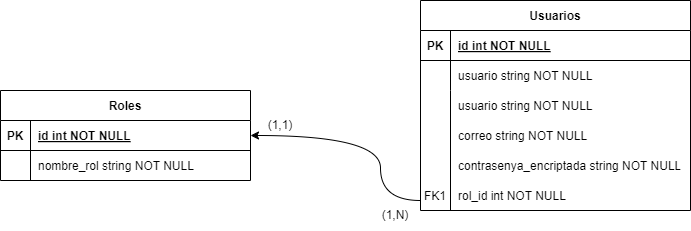
\includegraphics[width=0.9\linewidth]{Imagenes/Diagrama relacional.png}
    \caption{Diagrama Relacional}
    \label{Diagrama Relacional}
\end{figure}
\FloatBarrier

\section{Diseño procedimental}
En este apartado se van a mostrar mediante diagramas de flujo algunos de los procedimientos internos más interesantes y de mayor complejidad de este proyecto.

En el diagrama de flujo de la figura \ref{Diagrama de flujo Web scraping Frontend} podemos apreciar todos los pasos que se realizan cuando un usuario quiere obtener un libro a través del web scraping desde el \textit{frontend}. En la figura \ref{Diagrama de flujo permisos Backend} se aprecia la parte del \textit{backend}, donde se ejecuta toda la lógica

\newpage
\subsubsection{\textit{Frontend}:}
\begin{figure}[htbp]
    \centering
    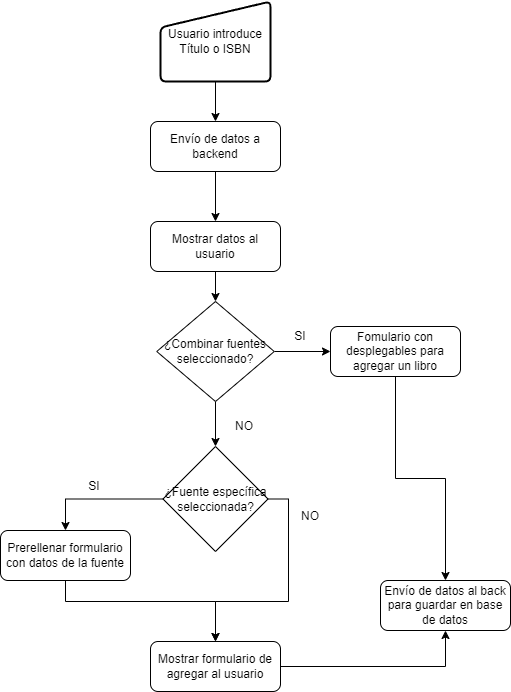
\includegraphics[width=0.7\linewidth]{Imagenes/Front web scraping.png}
    \caption{Diagrama de flujo Web scraping \textit{Frontend}}
    \label{Diagrama de flujo Web scraping Frontend}
\end{figure}
\FloatBarrier

\newpage
\subsubsection{\textit{Backend}:}
\begin{figure}[htbp]
    \centering
    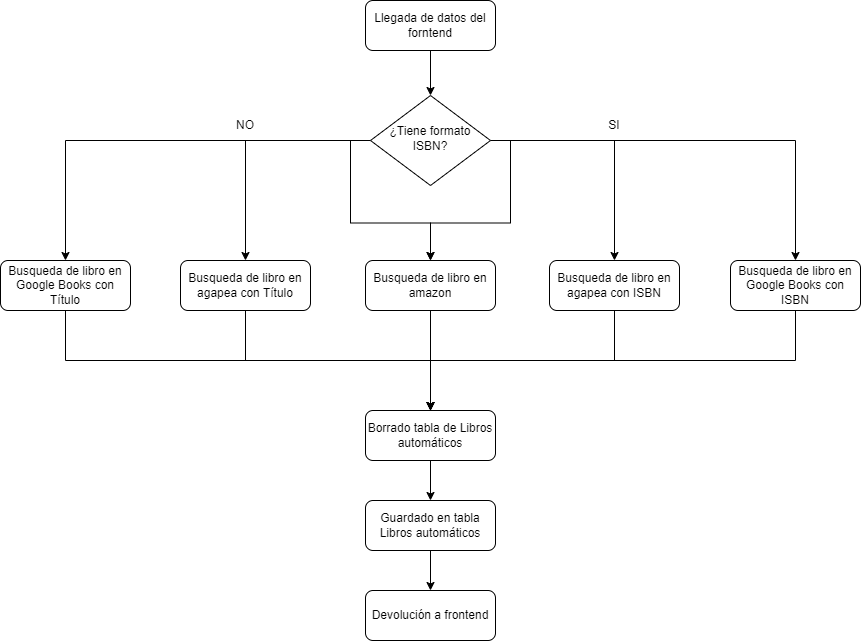
\includegraphics[width=1\linewidth]{Imagenes/Back web scraping.png}
    \caption{Diagrama de flujo Web scraping \textit{Backend}}
    \label{Diagrama de flujo Web scraping Backend}
\end{figure}
\FloatBarrier

En las figuras \ref{Diagrama de flujo permisos Frontend} y \ref{Diagrama de flujo permisos Backend} muestra el sistema que permite a la web bloquear o permitir la entrada dinámicamente a los usuarios a ciertas partes de la web utilizando permisos, los cuales no son estáticos y son editables.

\newpage
\subsubsection{\textit{Frontend}:}
\begin{figure}[htbp]
    \centering
    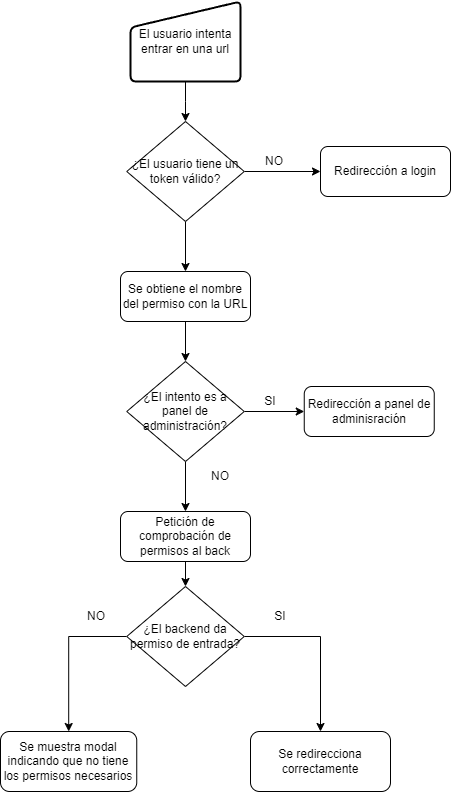
\includegraphics[width=0.6\linewidth]{Imagenes/Front permisos.png}
    \caption{Diagrama de flujo permisos \textit{Frontend}}
    \label{Diagrama de flujo permisos Frontend}
\end{figure}
\FloatBarrier

\newpage
\subsubsection{\textit{Backend}:}
\begin{figure}[htbp]
    \centering
    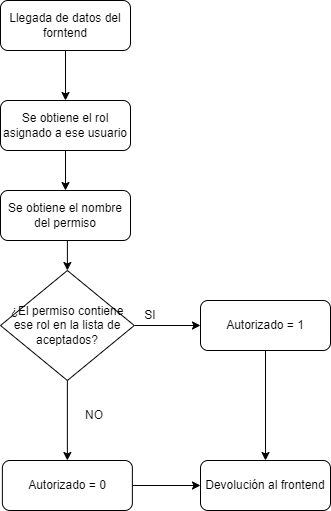
\includegraphics[width=0.5\linewidth]{Imagenes/Back permisos.png}
    \caption{Diagrama de flujo permisos \textit{Backend}}
    \label{Diagrama de flujo permisos Backend}
\end{figure}
\FloatBarrier

\section{Diseño de interfaces}
 Para realizar un primer prototipado del diseño de interfaz de la web se utilizó la herramienta Justimind, que ha permitido el diseño y la estructura de las funciones básicas de este proyecto.

A continuación, se muestran algunas de las interfaces realizadas con la herramienta:
\begin{figure}[htbp]
    \centering
    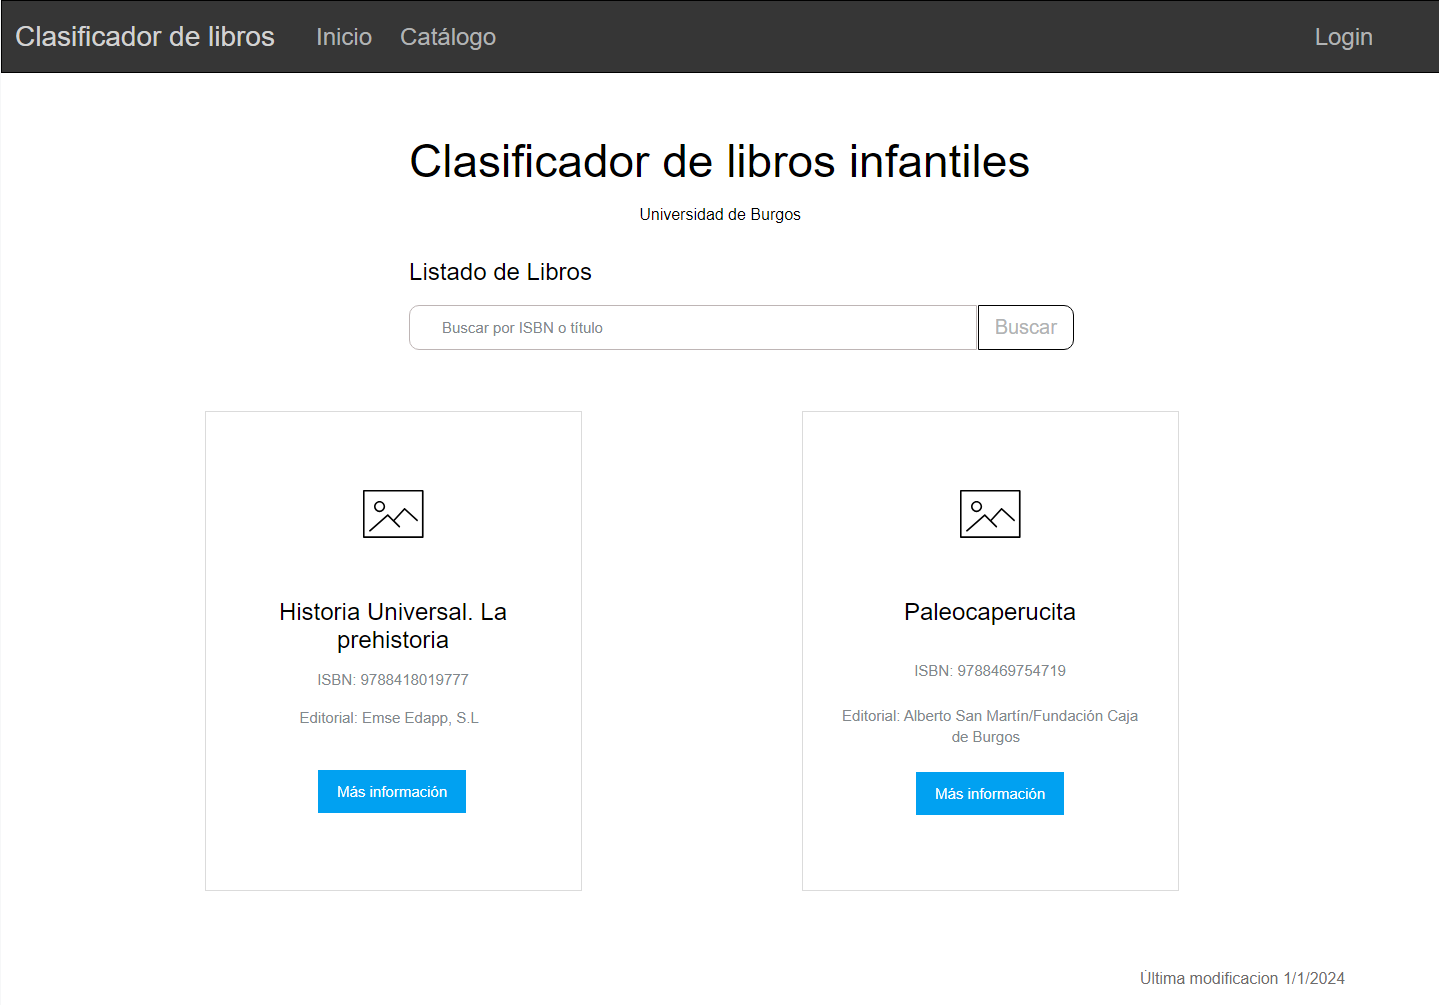
\includegraphics[width=0.9\linewidth]{Imagenes/PrototipoCatalogo.png}
    \caption{Prototipo catálogo}
    \label{Prototipo catálogo}
\end{figure}
\begin{figure}
    \centering
    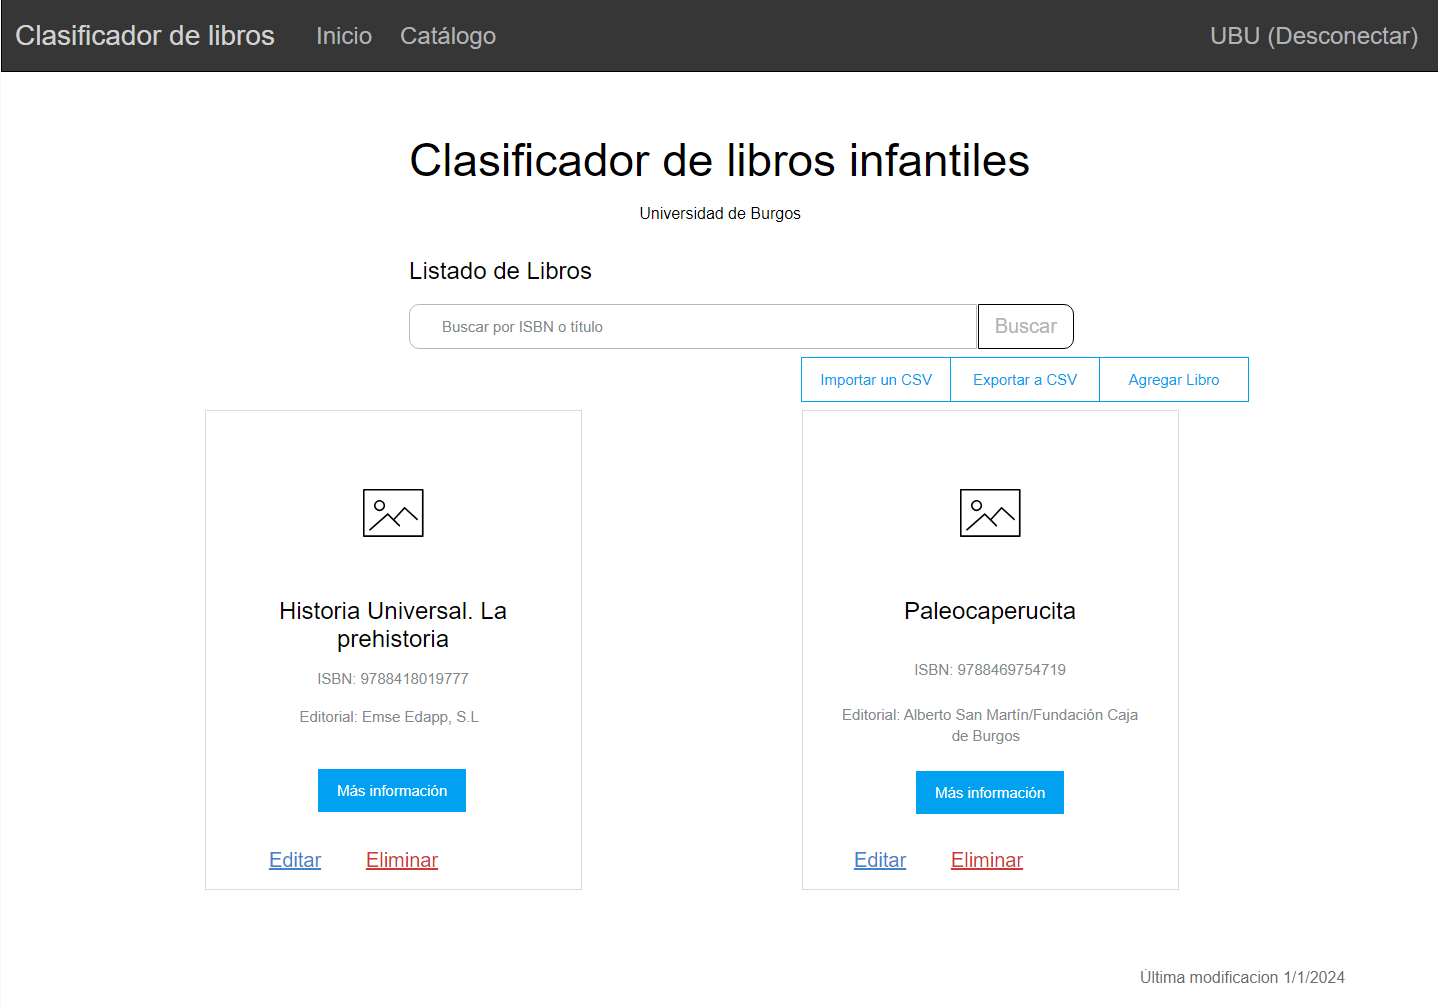
\includegraphics[width=0.9\linewidth]{Imagenes/CatalogoAdministrador.png}
    \caption{Prototipo catálogo (Vista de administrador)}
    \label{Prototipo catálogo (Vista de administrador)}
\end{figure}
\FloatBarrier

\begin{figure}[htbp]
    \centering
    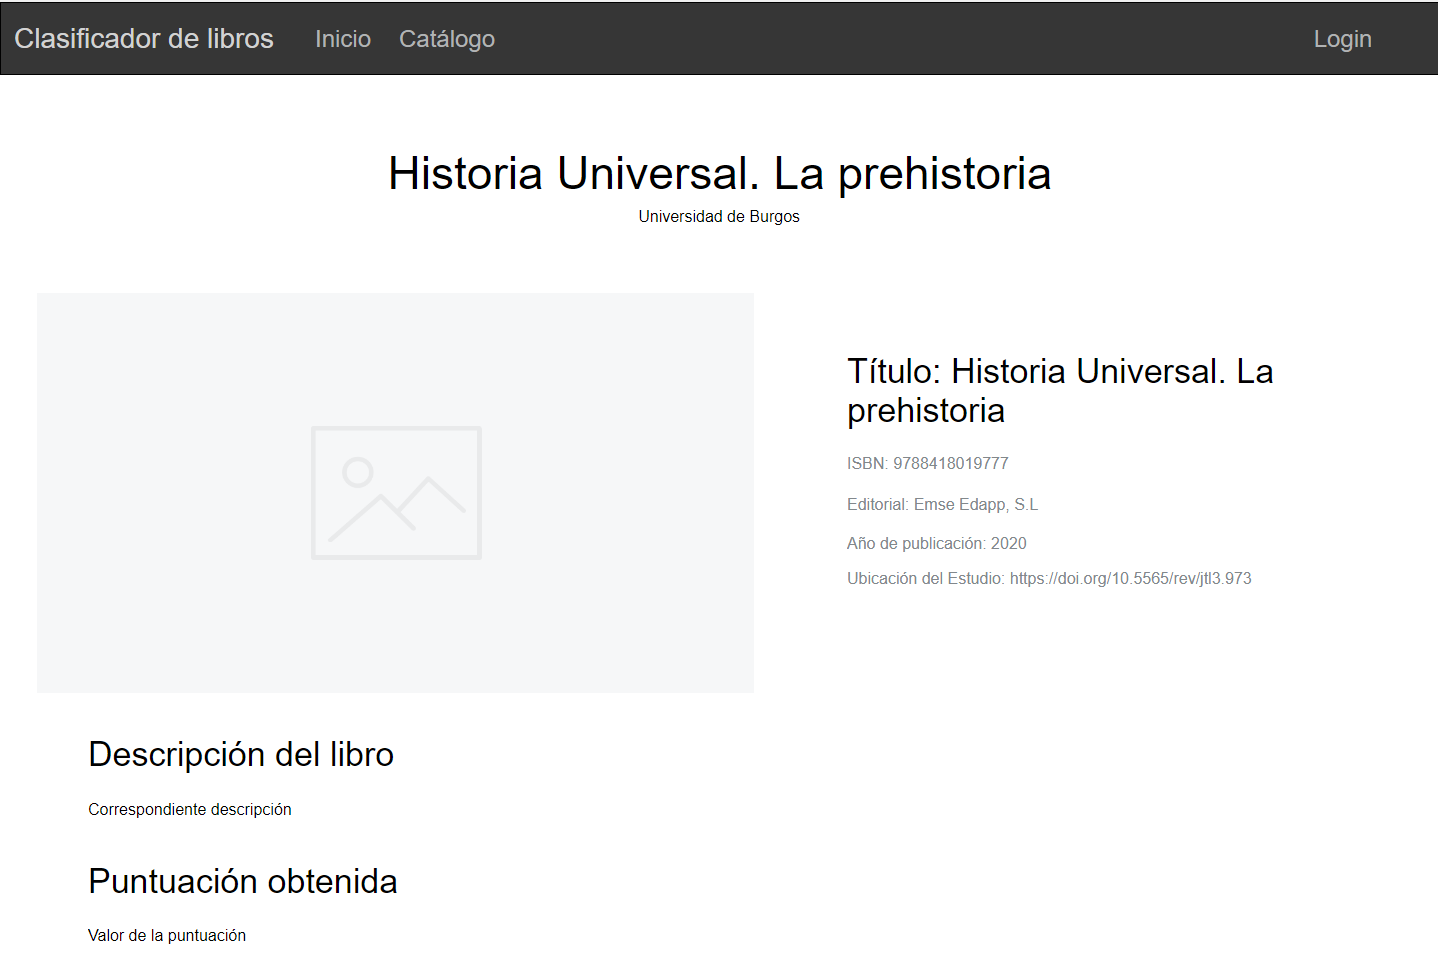
\includegraphics[width=0.9\linewidth]{Imagenes/PrototipoMasInfo.png}
    \caption{Prototipo Más Información}
    \label{Prototipo Más Información}
\end{figure}
\begin{figure}
    \centering
    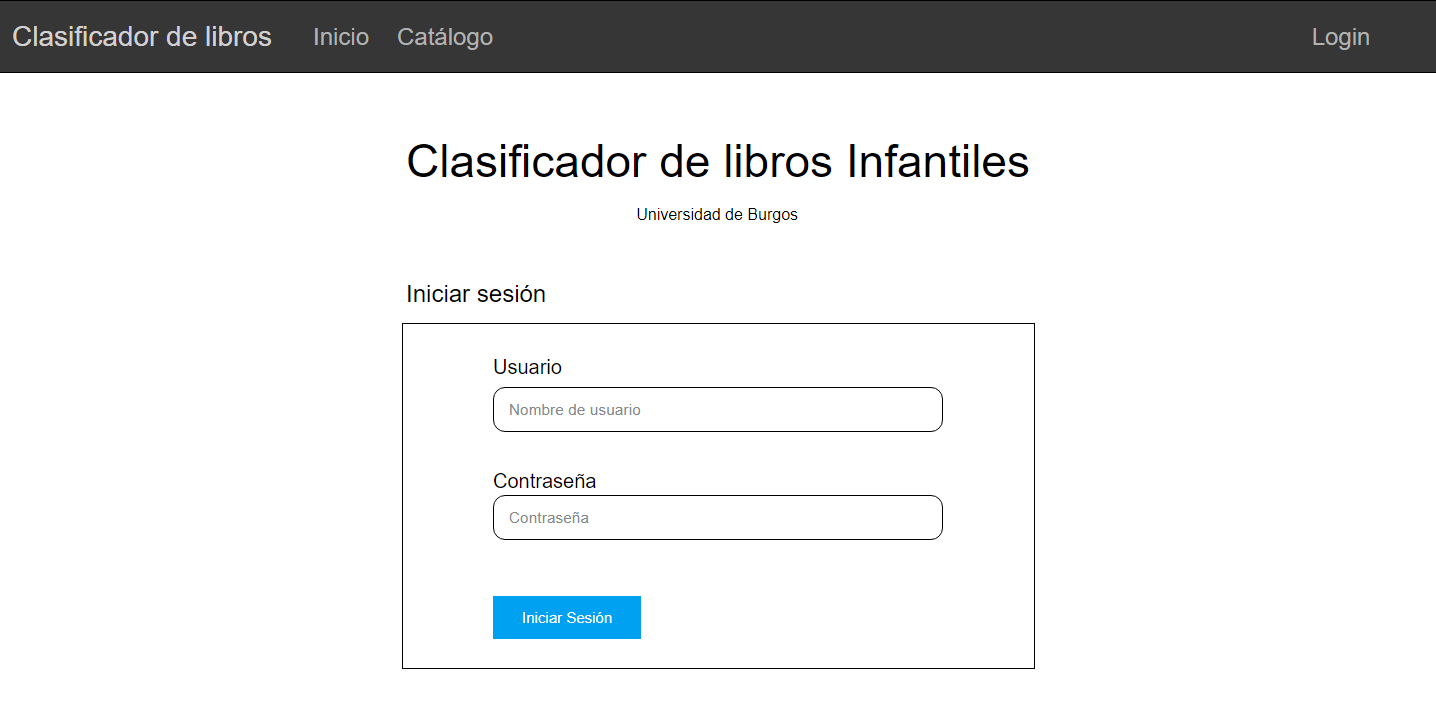
\includegraphics[width=0.9\linewidth]{Imagenes/PrototipoLogin.png}
    \caption{Prototipo Login}
    \label{Prototipo Login}
\end{figure}
\FloatBarrier

\section{Diseño de la arquitectura}
Dentro de este apartado se exponen los patrones de diseño utilizados durante el desarrollo de esta aplicación web. Para una mejor comprensión se separan los patrones de \textit{frontend} y \textit{backend} y finalmente la combinación de ambos.
\subsection{ Patrones del \textit{backend}}
\subsubsection{Patrón modular~\cite{PatrónMódulo}}
El patrón modular tiene como objetivo principal separar las funcionalidades del código en módulos separados y lo más independientes posibles. Cada módulo consiste en una o varias funcionalidades relacionadas entre sí. Esto contiene la gran ventaja de poder reutilizar el código y tener una escalabilidad y mantenibilidad muy simple y eficaz.

A nivel de ejemplo del \textit{backend}, en la figura \ref{Módulos backend} se puede apreciar cómo las funcionalidades principales se encuentran separadas en carpetas con sus correspondientes archivos, utilizando uno general para conectarlos entre si y poder usar todos los componentes.

\begin{figure}
    \centering
    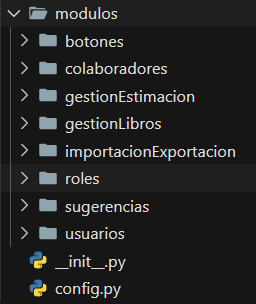
\includegraphics[width=0.5\linewidth]{Imagenes/Modulos.png}
    \caption{Módulos \textit{backend}}
    \label{Módulos backend}
\end{figure}


Un ejemplo más concreto de estos módulos es la carpeta gestionLibros, la cual es la encargada de toda la lógica relacionada con todas las operaciones del catálogo.

\begin{figure}[htbp]
    \centering
    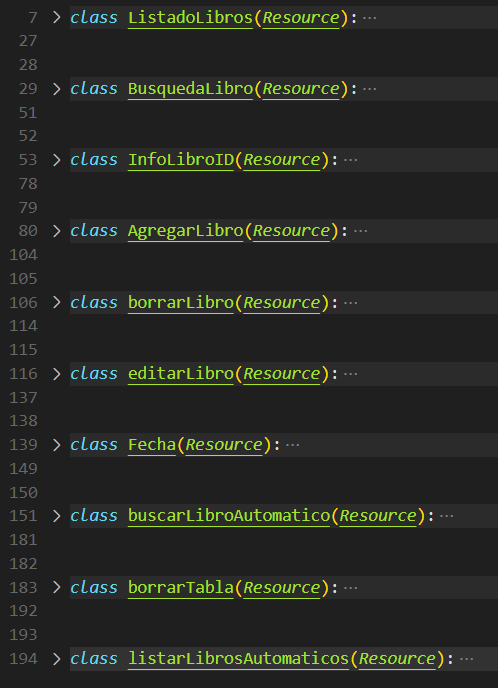
\includegraphics[width=0.5\linewidth]{Imagenes/Ejemplo gestionLibros.png}
    \caption{Funciones gestionLibros}
    \label{Funciones gestionLibros}
\end{figure}
\FloatBarrier

\subsubsection{Patrón repositorio\cite{PatrónRepositorio}}
El patrón repositorio es utilizado para permitir la separación entre el acceso a los datos de la base de datos con la lógica de negocio. Al realizar esta acción podemos tener grandes ventajas como son la limpieza, la mantenibilidad y la posibilidad de realización de pruebas unitarias de manera sencilla.

A nivel de ejemplo esto se puede apreciar en la estructura del proyecto al existir una separación entre todas los módulos de funcionalidades y el apartado de modelos.

\begin{figure}[htbp]
    \centering
    \includegraphics[width=0.4\linewidth]{Imagenes/Patrón repositorio.png}
    \caption{Patrón repositorio}
    \label{Patrón repositorio}
\end{figure}
\FloatBarrier

\subsection{Patrones del \textit{frontend}}
\subsubsection{Patrón de componentes~\cite{PatrónComponentes}}
El patrón de componentes consiste en dividir la interfaz del usuario en elementos totalmente independientes y reutilizables. Cada componente existente en el proyecto contiene su propia lógica y su propia y diseño, lo cual permite tener una modularización completa y muy fácilmente escalable. Este patrón es esencial para poder construir vistas muy complejas utilizando componentes muy pequeños.

Para ejemplificarlo, en la figura \ref{ComponentesAngular} se puede observar algunos de los componentes creados para la aplicación web, donde se observa la separación completa y los elementos de cada componente.
\begin{figure}
    \centering
    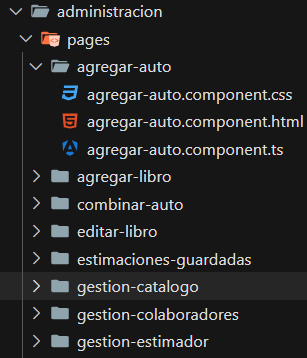
\includegraphics[width=0.4\linewidth]{Imagenes/ComponentesAngular.png}
    \caption{ComponentesAngular}
    \label{ComponentesAngular}
\end{figure}
\FloatBarrier

\subsubsection{Patrón de servicios~\cite{PatrónServicios}}
El patrón de servicios consiste en generar archivos que contengan la lógica que sea compartida por varios de los componentes. En el caso de este proyecto, los servicios se han utilizado para realizar las llamadas necesarias al \textit{backend}, definiendo así una serie de funciones que pueden compartir varios de los componentes existentes, en base a sus necesidades.
Para poder utilizar correctamente estos elementos, han de inyectarse en los constructores de todos aquellos componentes que quieran interactuar con ellos.

A modo de ejemplo, en la figura \ref{Servicio de libros} se puede ver una parte de uno de los servicios existentes (en este caso es el servicio de los libros), donde entre todos los elementos que contiene, se pueden observar las funciones que realizan las llamadas al \textit{backend} y una función donde se establecen las cabeceras de todas las llamadas.

\begin{figure}[htbp]
    \centering
    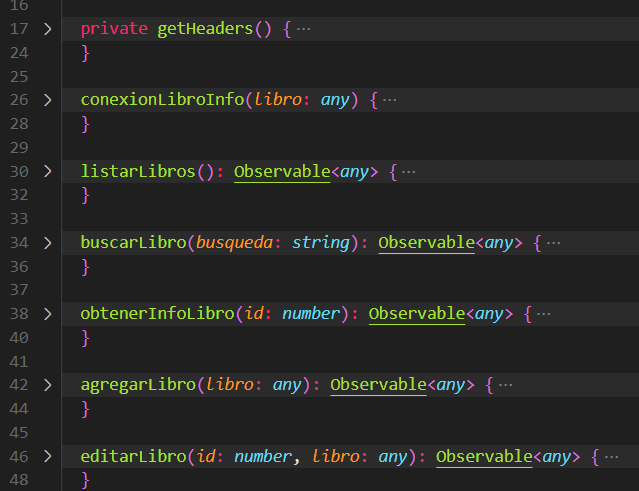
\includegraphics[width=0.7\linewidth]{Imagenes/LibroService.png}
    \caption{Servicio de libros}
    \label{Servicio de libros}
\end{figure}
\FloatBarrier

\newpage
\subsection{Patrones conjuntos}
\subsubsection{Patrón cliente-servidor~\cite{ModeloClienteServidor}}
Este último patrón es uno de los más importantes de este proyecto y se genera al existir de manera separada el \textit{backend} y el \textit{frontend}.
La forma en la que se muestra este patrón es de la siguiente manera:
\begin{itemize}
    \item Cliente: El cliente es el responsable de la interfaz de usuario, y en este proyecto recaería sobre la parte de Angular.
    \item Servidor: Son los responsables de devolver los recursos pedidos por los clientes, por lo que esta parte recaería sobre el \textit{backend} Flask.
\end{itemize}

El funcionamiento de este patrón se realiza mediante solicitudes HTTP por parte del cliente al servidor, los cuáles recibe el \textit{backend}, que procesa la información pedida utilizando parámetros recibidos del cliente (si existieran), y devuelve un resultado para que el cliente lo procese.



\apendice{Documentación técnica de programación}

\section{Introducción}
Este anexo contiene toda la información técnica de programación, incluyendo la estructura de directorios, las instalaciones necesarias, el proceso de arranque de la aplicación y los test generados. Esto es de gran utilidad para todo desarrollador/a que quiera realizar modificaciones al proyecto actual.
\section{Estructura de directorios}
\subsection{Estructura de directorios del \textit{frontend}}

\begin{itemize}
    \item \texttt{frontendAngular/}
    \begin{itemize}
        \item \texttt{.angular/} -- Archivos de configuración específica de Angular.
        \item \texttt{dist/} -- Archivos generados después de la construcción del proyecto.
        \item \texttt{node\_modules/} -- Dependencias de Node.js instaladas.
        \item \texttt{src/} -- Directorio principal de código fuente.
        \begin{itemize}
            \item \texttt{app/}
            \begin{itemize}
                \item \texttt{administracion/} -- Páginas específicas de la administración y su módulo.
                
                \item \texttt{aplicacion/} -- Páginas específicas de la administración y su módulo.
                \item \texttt{auth/} -- Módulo y componentes de autenticación.
                \item \texttt{prime-ng/} -- Configuración del módulo PrimeNG.
                \item \texttt{services/} -- Servicios que manejan la lógica de negocio y comunicación con la API.
                \item \texttt{shared/} -- Componentes compartidos en varios componentes.
                \item \texttt{app-routing.module.ts} -- Configuración de rutas de la aplicación.
                \item \texttt{app.component.css} -- Estilos del componente principal de la aplicación.
                \item \texttt{app.component.html} -- Plantilla HTML del componente principal.
                \item \texttt{app.component.ts} -- Lógica del componente principal.
                \item \texttt{app.module.ts} -- Módulo principal de la aplicación.
            \end{itemize}
            \item \texttt{assets/} -- Recursos estáticos de la aplicación (Imágenes).
            \begin{itemize}
                \item \texttt{.redirects} -- Configuración de redirecciones para Netlify.
                \item \texttt{index.html} -- Página principal de la aplicación.
                \item \texttt{main.ts} -- Punto de entrada principal de la aplicación.
                \item \texttt{styles.css} -- Estilos globales de la aplicación.
                \item \texttt{.editorconfig} -- Configuración del editor.
            \end{itemize}
        \end{itemize}
        \item \texttt{.gitignore} -- Archivos y directorios a ignorar por Git.
        \item \texttt{angular.json} -- Configuración del proyecto Angular.
        \item \texttt{package-lock.json} -- Descripción detallada de las dependencias instaladas.
        \item \texttt{package.json} -- Configuración y dependencias del proyecto.
        \item \texttt{README.md} -- Documentación del proyecto.
        \item \texttt{tsconfig.app.json} -- Configuración de TypeScript para la aplicación.
        \item \texttt{tsconfig.json} -- Configuración global de TypeScript.
        \item \texttt{tsconfig.spec.json} -- Configuración de TypeScript para pruebas.
    \end{itemize}
\end{itemize}


\subsection{Estructura de directorios del \textit{backend}}

\begin{itemize}
    \item \texttt{API PYTHON/}
    \begin{itemize}
        \item \texttt{app/} -- Directorio principal del código fuente de la aplicación.
        \begin{itemize}
            \item \texttt{Funciones\_Auxiliares/} -- Funciones auxiliares utilizadas en la aplicación.
            \begin{itemize}
                \item \texttt{automatizar\_correo.py} -- Script para automatizar el envío de correos.
                \item \texttt{funciones\_webscraping.py} -- Funciones para realizar web scraping.
            \end{itemize}
            \item \texttt{modelos/} -- Definición de modelos de datos.
            \begin{itemize}
                \item \texttt{\_\_init\_\_.py} -- Inicialización del paquete de modelos.
                \item \texttt{modelos.py} -- Definición de los modelos de la base de datos.
            \end{itemize}
            \item \texttt{modulos/} -- Módulos de la aplicación, organizados por funcionalidad.
            \begin{itemize}
                \item \texttt{botones/} -- Módulo con la funcionalidad de botones y permisos.
                \item \texttt{colaboradores/} -- Módulo con la gestión de colaboradores.
                \item \texttt{gestionEstimacion/} -- Módulo con la gestión de estimaciones.
                \item \texttt{gestionLibros/} -- Módulo con la gestión de libros.
                \item \texttt{importacionExportacion/} -- Módulo con la importación y exportación del catálogo.
                \item \texttt{roles/} -- Módulo con la gestión de roles de usuarios.
                \item \texttt{sugerencias/} -- Módulo con la gestión de sugerencias.
                \item \texttt{usuarios/} -- Módulo con la gestión de usuarios.
                \item \texttt{\_\_init\_\_.py} -- Inicialización del paquete de módulos.
            \end{itemize}
            \item \texttt{config.py} -- Archivo de configuración de la aplicación.
        \end{itemize}
        \item \texttt{instance/} -- Directorio de la base de datos local.
        \item \texttt{tests/} -- Directorio que contiene las pruebas unitarias.
        \item \texttt{requirements.txt} -- Archivo que lista las dependencias del proyecto.
        \item \texttt{run.py} -- Script para iniciar la aplicación.
    \end{itemize}
\end{itemize}

\section{Manual del programador}
Este manual tiene como objetivo formar a todo aquel que desee realizar desarrollos o modificaciones a este proyecto. En él se explican las instalaciones necesarias para generar el entorno de desarrollo, obtener el código, y una guía para ejecutarlo.

\subsection{Instalaciones necesarias}
Para este proyecto se requieren realizar las siguientes instalaciones:
\begin{itemize}
    \item Visual Studio Code
    \item Git
    \item NodeJS 20.11.1
    \item Python 3.12.1
\end{itemize}

\subsubsection{Visual Studio Code}
Este a sido el editor de código elegido para realizar este proyecto, por lo que es recomendable usarle por su facilidad de configuración y variedad de extensiones útiles.
Para instalar este editor de código debemos dirigirnos a la página oficial
\href{https://code.visualstudio.com/}{Visual Studio Code} y descargarnos la última versión estable.
\begin{figure}[h]
    \centering
    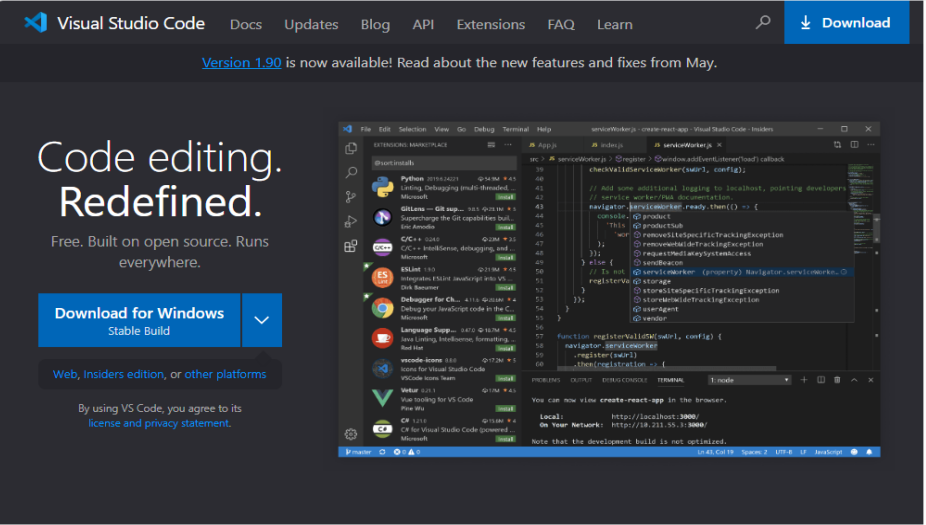
\includegraphics[width=0.75\linewidth]{Imagenes/VisualInstalacion.png}
    \caption{Página de instalación de Visual Studio Code}
    \label{Página de instalación de Visual Studio Code}
\end{figure}
\FloatBarrier


Una vez se nos descarga el instalador se mantienen las opciones por defecto y se procede a la instalación. Una vez instalado es recomendable dirigirse al apartado de extensiones e instalar las siguientes:
\begin{itemize}
    \item Angular Language Service
    \item Angular 17 Snippets
    \item Angular Schematics
    \item angular2-inline
    \item TypeScript Importer
    \item Python (Automáticamente instala las dos siguientes)
    \item Pylance
    \item Python Debugger
\end{itemize}

Además de esas, existen extensiones opcionales pero muy recomendables:
\begin{itemize}
    \item Error Lens
    \item Better Comments
    \item Material Icon Theme
    \item Auto Close Tag
    \item Activitus Bar
\end{itemize}

Si todos estos pasos se han realizado correctamente, deberíamos tener el Visual Studio iniciado correctamente y 13 extensiones instaladas.


\begin{figure}[h]
    \centering
    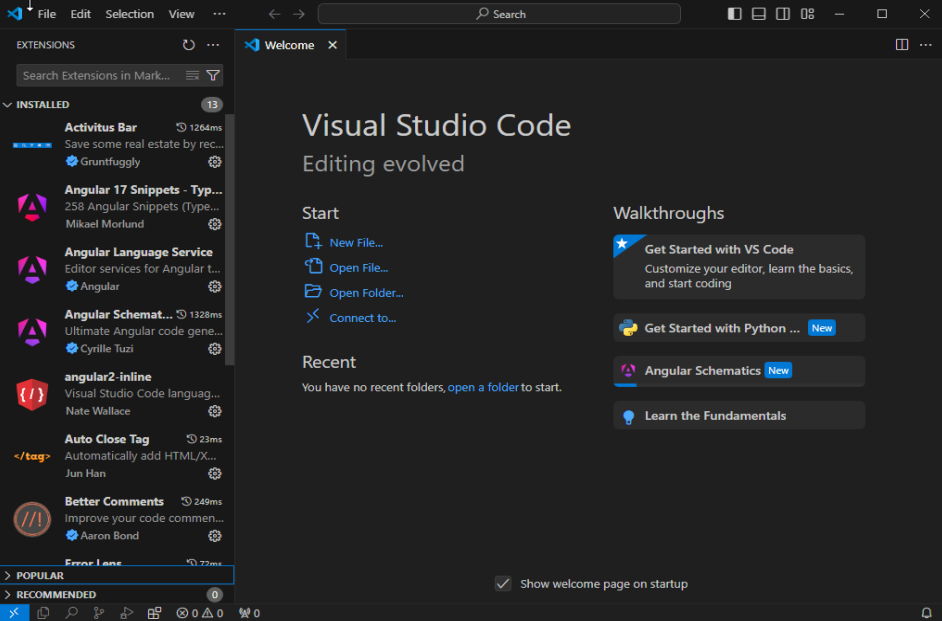
\includegraphics[width=0.75\linewidth]{Imagenes/ExtensionesVisual.png}
    \caption{Extensiones instaladas Visual Studio Code}
    \label{Extensiones instaladas Visual Studio Code}
\end{figure}
\FloatBarrier

\subsubsection{Python}

Este lenguaje es el usado para el \textit{backend} con la versión 3.12.1, por lo que para instalar esta versión debemos de dirigirnos a la web oficial de Python y seleccionar esa versión (\href{https://www.python.org/downloads/release/python-3121/}{Versión 3.12.1 de python}).
En la parte de abajo de esta página se encuentran todas las opciones de instalación, en este caso se va a escoger el instalador de Windows 64x ya que es el sistema operativo utilizado.
Una vez abierto el instalador, es recomendable activar la checkbox que agrega python.exe al PATH, ya que si no se encuentra activo puede acarrear problemas en el futuro.
Una vez seleccionamos esa opción, pulsamos en instalar ahora para que proceda con la instalación.

\begin{figure}[h]
    \centering
    \includegraphics[width=0.75\linewidth]{Imagenes/InstalaciónPython.png}
    \caption{Instalador de Python}
    \label{Instalador de Python}
\end{figure}
\FloatBarrier

\subsubsection{NodeJS}
NodeJS es el encargado de compilar el lenguaje TypeScript utilizado en Angular así como el administrados de dependencias del proyecto en la parte \textit{frontend}. En Prehistoria en Igualdad se ha utilizado la versión 20.11.1, la cual se instala desde esta URL \href{https://nodejs.org/en/blog/release/v20.11.1}{Versión 20.11.1 de node}

Ya dentro de la web de NodeJS bajamos en la página y encontramos la zona de instaladores. En este caso se instala la versión de Windows 64 bit en formato instalador.

Una vez abierto el instalador, se va dando al botón de siguiente aceptando las condiciones y el resto de campos se dejan por defecto.
Si tras la instalación, no sale en el instalador que se ha instalado correctamente, no es necesario realizar más pasos.

\begin{figure}[h]
    \centering
    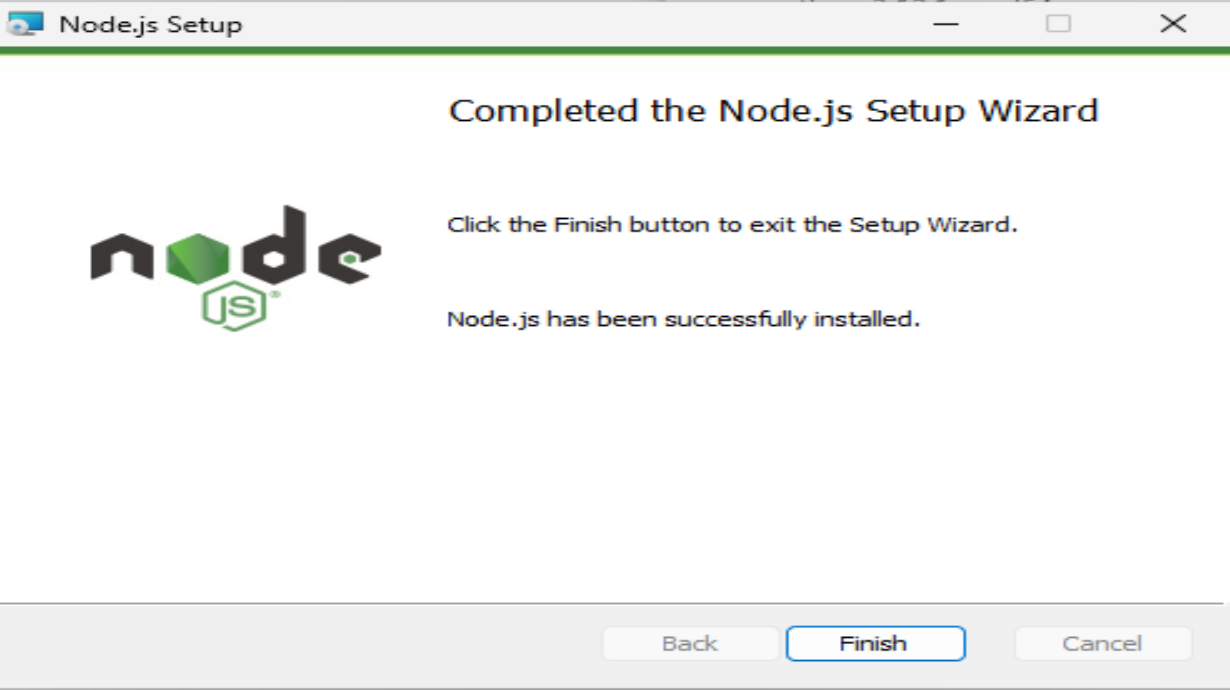
\includegraphics[width=0.75\linewidth]{Imagenes/InstaladorNode.png}
    \caption{Instalación existosa de NodeJS}
    \label{Instalación existosa de NodeJS}
\end{figure}
\FloatBarrier

\subsubsection{Git}
Git es una herramienta de control de versiones que se ha utilizado en este proyecto para ir actualizando los cambios en GitHub y que en este manual se va a utilizar para obtener el proyecto del repositorio para poder ejecutarlo desde local.
La instalación de Git comienza en la \href{https://www.git-scm.com/downloads}{página oficial}, donde descargaremos su instalador con la versión más reciente en la versión \textit{Standalone}.

Una vez descargado el instalador, nos pedirá por permisos de administración el poder realizar cambios. Una vez aceptado, se dejan todas las opciones por defecto y se da al botón de continuar para que se ejecute la instalación.

Si se ha instalado correctamente, al cerrar el instalador nos dará la opción de ver las últimas modificaciones de esta versión.


\subsection{Obtención del código fuente y Ejecución del código}
Para obtener el código del proyecto existen varias vías, pero en este caso se va a utilizar la herramienta ya instalada Git.

Con los comandos que se muestran a continuación se podrá descargar de manera rápida todos los ficheros.
\begin{itemize}
    \item Abrimos una terminal de Git en el directorio en el que queramos guardar el proyecto.
    \begin{figure}[h]
        \centering
        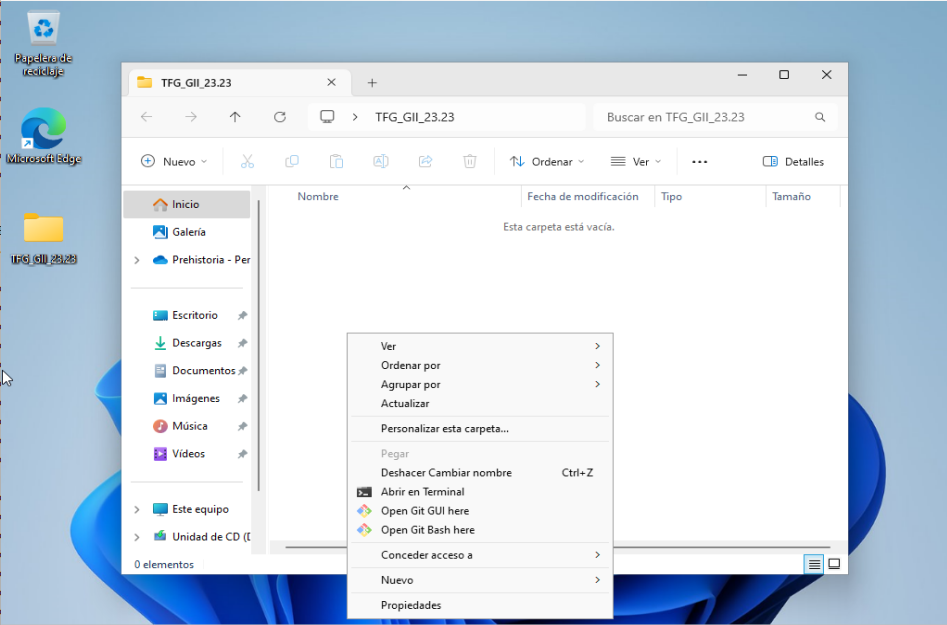
\includegraphics[width=0.75\linewidth]{Imagenes/AperturaTerminalGit.png}
        \caption{Apertura de terminal Git}
        \label{Apertura de terminal Git}
    \end{figure}
    \FloatBarrier
    \item Introducimos los siguientes comandos con la información personal:
    \begin{enumerate}
        \item git config --global user.name "Tu Nombre"
        \item git config --global user.email "tuemail@example.com"
    \end{enumerate}

    \begin{figure}[h]
        \centering
    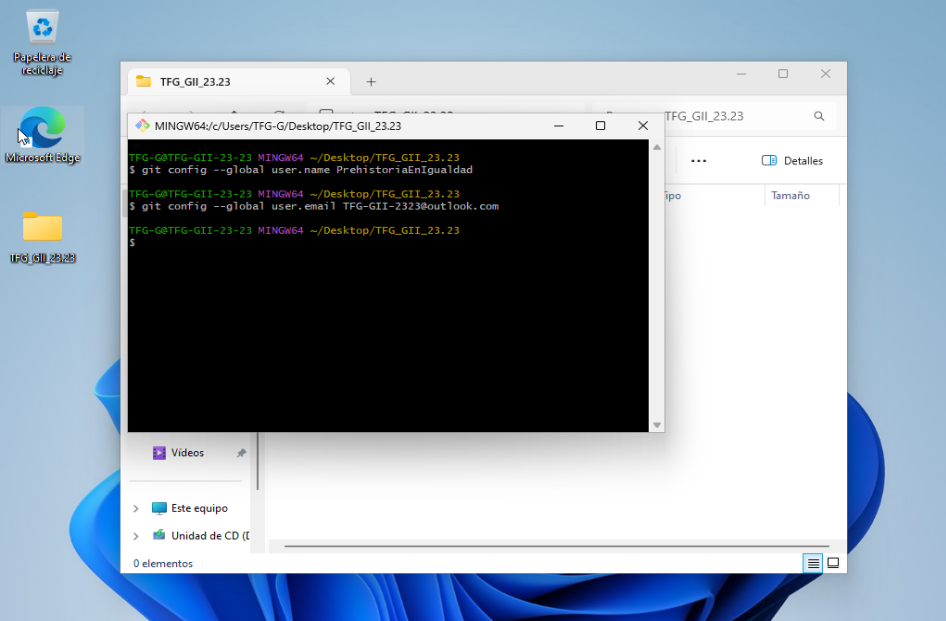
\includegraphics[width=1\linewidth]{Imagenes/ComandosUsuarioCorreoGit.png}
        \caption{Comandos de Usuario y correo de Git}
        \label{Comandos de Usuario y correo de Git}
    \end{figure}
    \FloatBarrier
    \item Ejecutamos el comando que clona el repositorio en local.
    \begin{enumerate}
        \item git clone https://github.com/DanielFernandezFdez/TFG\_GII\_23.23.git
    \end{enumerate}

    \begin{figure}[h]
        \centering
        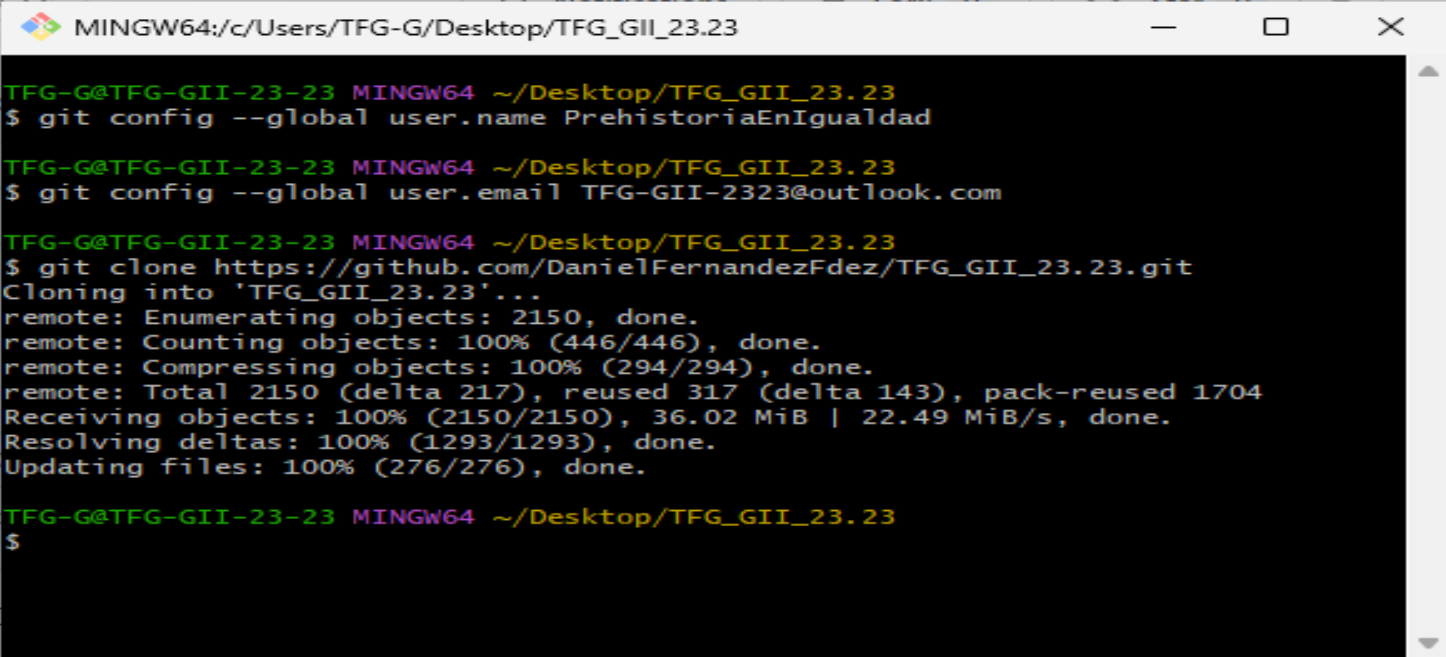
\includegraphics[width=0.75\linewidth]{Imagenes/GitClone.png}
        \caption{Clonación del repositorio}
        \label{Clonación del repositorio}
    \end{figure}
    \FloatBarrier
\end{itemize}


Una vez importado correctamente, desde visual le damos a abrir carpeta y seleccionamos el proyecto que acabamos de obtener.

Antes de comenzar con la ejecución, han de realizarse unos pasos previos para finalizar la instalación de dependencias.

\begin{itemize}
    \item Instalación de dependencias del \textit{backend}
    \begin{enumerate}
        \item Dentro de la carpeta 'API PYTHON' ejecutar el siguiente comando para generar un entorno virtual:

        python -m venv [Nombre del entorno]
        
        Si es satisfactoria la creación, dentro de la carpeta API PYTHON se generará una carpeta con el nombre dado.

        \item Activamos el entorno virtual para cargar las dependencias:

        [Nombre del entorno virtual]\textbackslash{Scripts}\textbackslash{Activate}

        Si se ha ejecutado correctamente nos tendría que aparecer el nombre en la línea de comandos entre paréntesis. En el caso de la figura \ref{Activar entorno virtual} se puede observar en la parte izquierda en color verde el nombre \texttt{EntornoVirtual}.

        \begin{figure}[h]
            \centering
            
\includegraphics[width=1\linewidth]{Imagenes/ActivarVenv.png}
            \caption{Activar entorno virtual}
            \label{Activar entorno virtual}
        \end{figure}
        \FloatBarrier
        
        \item Con el entorno virtual activo volcamos las dependencias del archivo requirements.txt con el comando:

        py -m pip install -r requirements.txt

        \item Con todos estos pasos realizados, con ejecutar el comando \textit{python run.py} se iniciaría el backend. Es importante recordar que hay que activar el entorno virtual antes de iniciar la API.
    \end{enumerate}

    \item Instalación de dependencias del \textit{frontend}
    \begin{enumerate}
        \item Situarnos en la carpeta frontendAngular con la consola.
        \item Ejecutar el comando \textit{npm install} para instalar las dependencias y el \textit{framework} Angular.
        \item Una vez terminada la descarga, podemos arrancar el frontend con el comando \textit{npm start}
    \end{enumerate}
\end{itemize}

\subsubsection{Cambiar la configuración de producción a local}
\begin{itemize}
    \item En la parte del \textit{backend}, en el fichero config.py cambiar la variable db\_path a la comentada.

    \item En la parte del \textit{frontend}, en los ficheros service, cambiar la variable apiURL a la comentada.
\end{itemize}

\section{Pruebas del sistema}
En esta última sección se describen las pruebas disponibles para comprobar si los cambios han generado resultados inesperados, y así poder solucionarlos antes de realizar el despliegue.

\subsection{Ejecutar}
\begin{enumerate}
    \item Abre una terminal o línea de comandos en el Visual Studio Code.
    \item Navega al directorio de la carpeta \texttt{tests}.
    \item Ejecuta el siguiente comando para ejecutar todas las pruebas unitarias:

    pytest [nombre del test]

    Este comando ejecutará todas las pruebas definidas en el archivo y generará un reporte con los resultados.
    Si se pone simplemente \textit{pytest ./} y ejecutará todos los test de la carpeta.

\end{enumerate}

\subsubsection{Resultados de las Pruebas}
Después de ejecutar las pruebas, \texttt{pytest} generará un reporte en la terminal mostrando qué pruebas pasaron y cuáles fallaron. Si alguna prueba falla, \texttt{pytest} proporcionará detalles sobre la causa del fallo, permitiéndote identificar y corregir el problema.

\subsection{Pruebas Manuales con Postman}

Además de las pruebas unitarias, se recomienda realizar pruebas manuales utilizando Postman para verificar el comportamiento de las APIs del sistema. Postman es una herramienta potente para probar y documentar APIs. A continuación se describe cómo utilizar Postman para realizar estas pruebas.

\subsubsection{Configuración de Postman}
Si aún no tienes Postman instalado, puedes descargarlo e instalarlo desde \href{https://www.postman.com/downloads/}{Postman}. Una vez instalado, sigue estos pasos:

\begin{enumerate}
    \item Abrir Postman.
    \item Agregar una nueva solicitud a la búsqueda con la URL local. Configurar el tipo de solicitud (GET, POST, PUT, DELETE).
    \item Configurar los parámetros necesarios, como headers y cuerpo en formato JSON.
    \item Envíar la solicitud y verificar la respuesta. Postman mostrará el código de estado HTTP y el cuerpo de la respuesta recibida del servidor.
\end{enumerate}

\subsubsection{Validación de Respuestas}
Para cada solicitud, hay que asegurarse que la respuesta recibida es la esperada. Esto incluye verificar:
\begin{itemize}
    \item El código de estado HTTP (por ejemplo, 200 OK, 404 Not Found, 500 Internal Server Error).
    \item El contenido del cuerpo de la respuesta, asegurando que los datos devueltos sean correctos y estén en el formato esperado.
    \item Los headers de la respuesta, si es necesario.
\end{itemize}

\apendice{Documentación de uso}

\section{Introducción}
En este manual se detallan los requisitos de la aplicación web para poder utilizarla correctamente así como su manual completo de uso de la aplicación dividido en dos partes. La primera de ellas muestra las opciones disponibles para una persona que no tenga cuenta en la aplicación, y la segunda muestra toda la parte que puede utilizar el personal de administración.
\section{Requisitos de uso}
Los requisitos mínimos de la aplicación web son los siguientes:
\begin{itemize}
    \item Conexión a internet
    \item Un navegador web para entrar a la siguiente URL: \href{https://prehistoriaenigualdad.netlify.app/}{Prehistoria en igualdad}
\end{itemize}
\section{Instalación}
En este caso no se necesita realizar ningún tipo de instalación, ya que en todos los dispositivos ya existe por defecto un navegador con el que poder entrar a la aplicación web.
\section{Manual del usuario/a sin cuenta}
En este apartado se recogen todas las acciones que puede realizar un usuario que no se encuentre registrado en la aplicación web.

\subsection{Consultar en el catálogo un libro}
Una de las funciones principales de esta aplicación es mostrar información a docentes y familias acerca de los libros analizados. Existen dos opciones para realizar esta operación.

\begin{enumerate}
    \item Desde el inicio.
    \begin{itemize}
        \item Rellenar el campo de búsqueda con un ISBN o con un Título.
        \item Automáticamente se redirige al catálogo con la búsqueda completada mostrando el libro deseado al hacer click en el botón de buscar.
    \end{itemize}
    \item Realizando la búsqueda desde el catálogo.
    \begin{itemize}
        \item Hacer click en el menú superior en el botón catálogo
        \item Rellenar el campo de búsqueda con ISBN o Título.
        \item Hacer click en la lupa para realizar la búsqueda.
        \item Se mostrarán los libros que coincidan con los parámetros de la búsqueda
    \end{itemize}
\end{enumerate}


\begin{figure}[h]
    \centering
    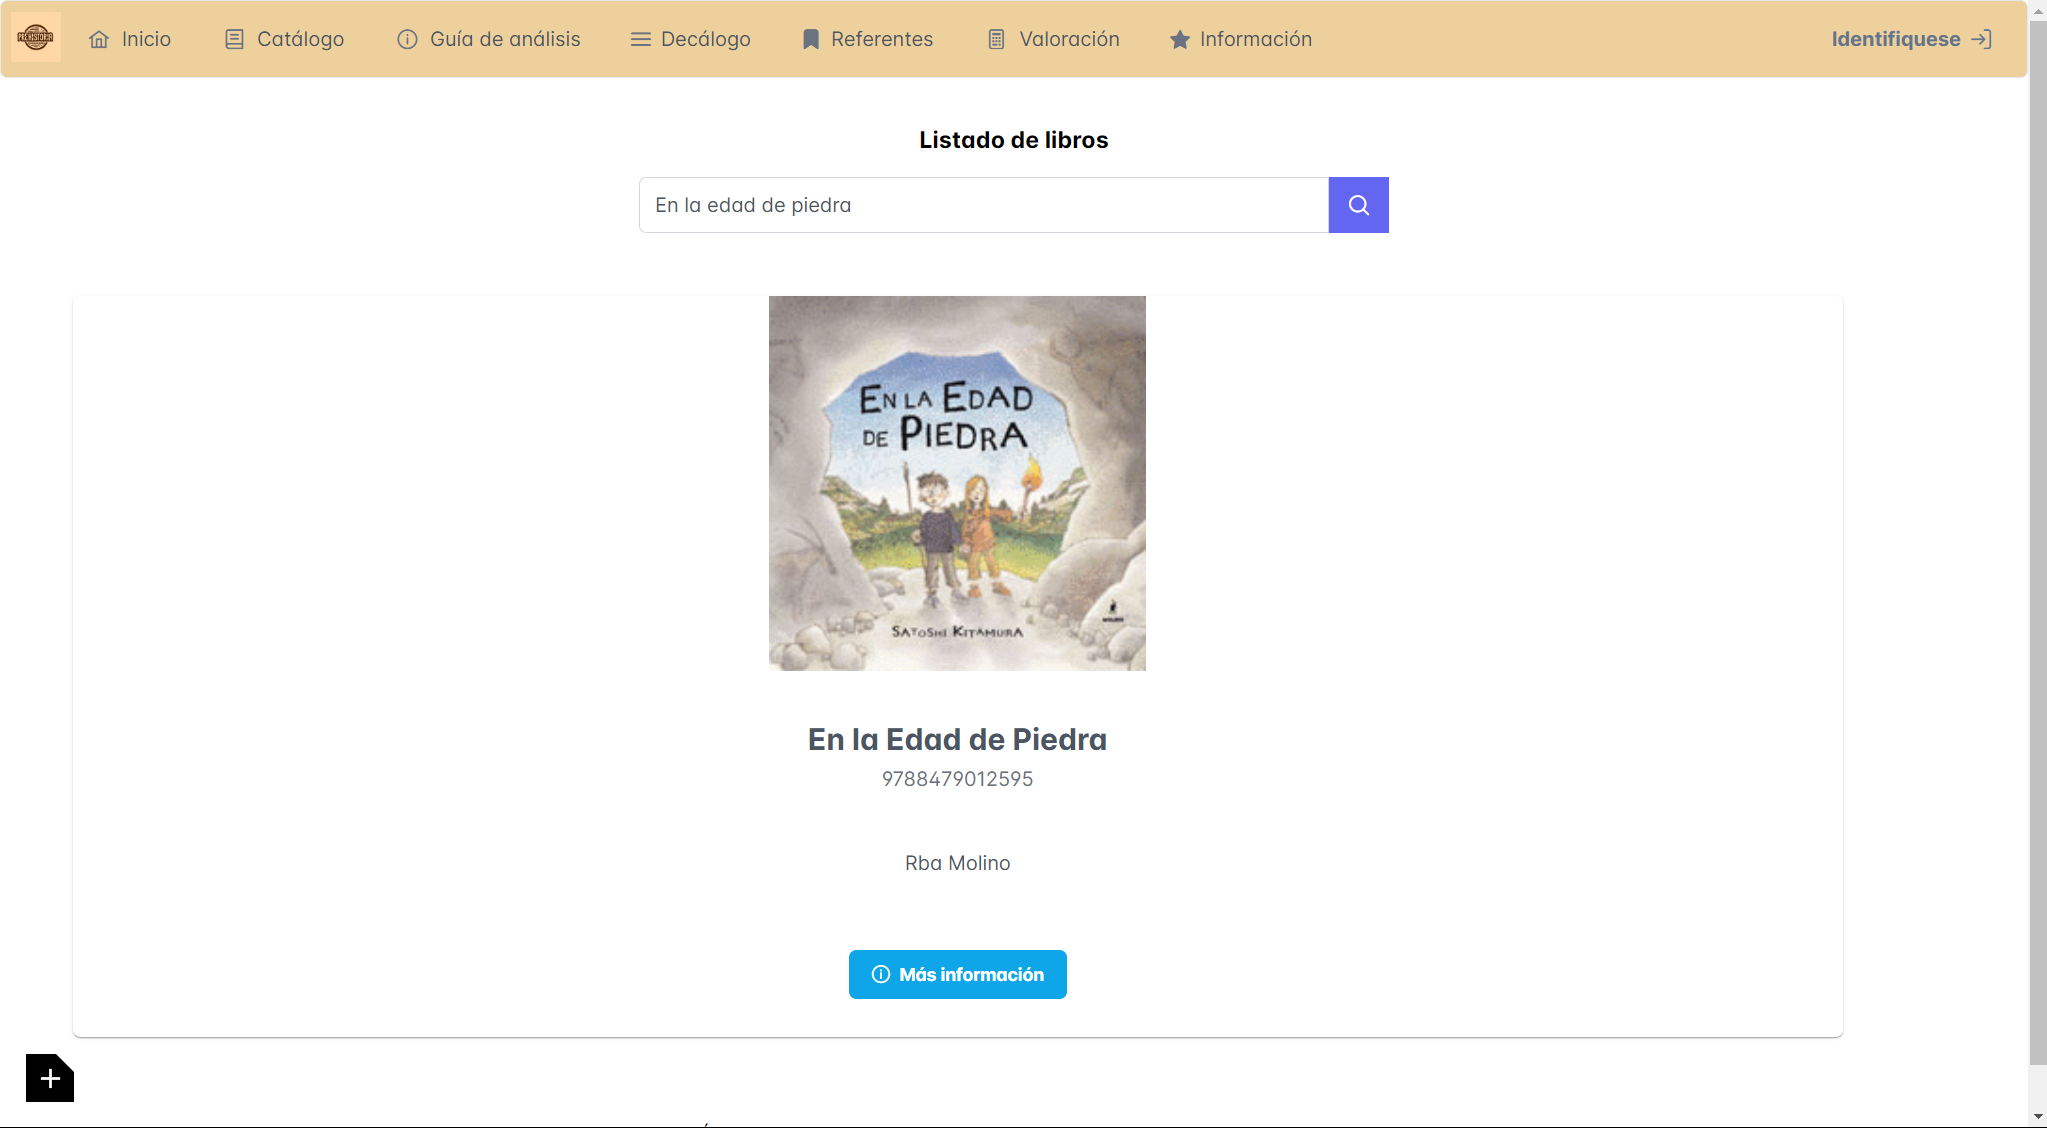
\includegraphics[width=1\linewidth]{Imagenes/ManualBusquedaLibro.png}
    \caption{Búsqueda de libro en catálogo}
    \label{Búsuqeda de libro en catálogo}
\end{figure}
\FloatBarrier

\subsection{Consultar la información de un libro}
Si un usuario/a conoce un libro sobre el que quiere consultar toda su información, se han de realizar los siguientes pasos. 

\begin{itemize}
    \item Buscar un libro desde inicio o desde el catálogo.
    \item Seleccionar el botón de más información del libro deseado.
    \item Hacer click en el botón de más información correspondiente a ese libro
\end{itemize}
Las acciones que se pueden realizar dentro de este apartado son los siguientes:
\begin{enumerate}
    \item Si se hace click en el símbolo de información, la web cargará la pestaña de la guía de análisis.
    \item El apartado de la ubicación del estudio, si contiene información, es un hipervínculo que lleva a la dirección del estudio de ese libro
\end{enumerate}
\begin{figure}[h]
    \centering
    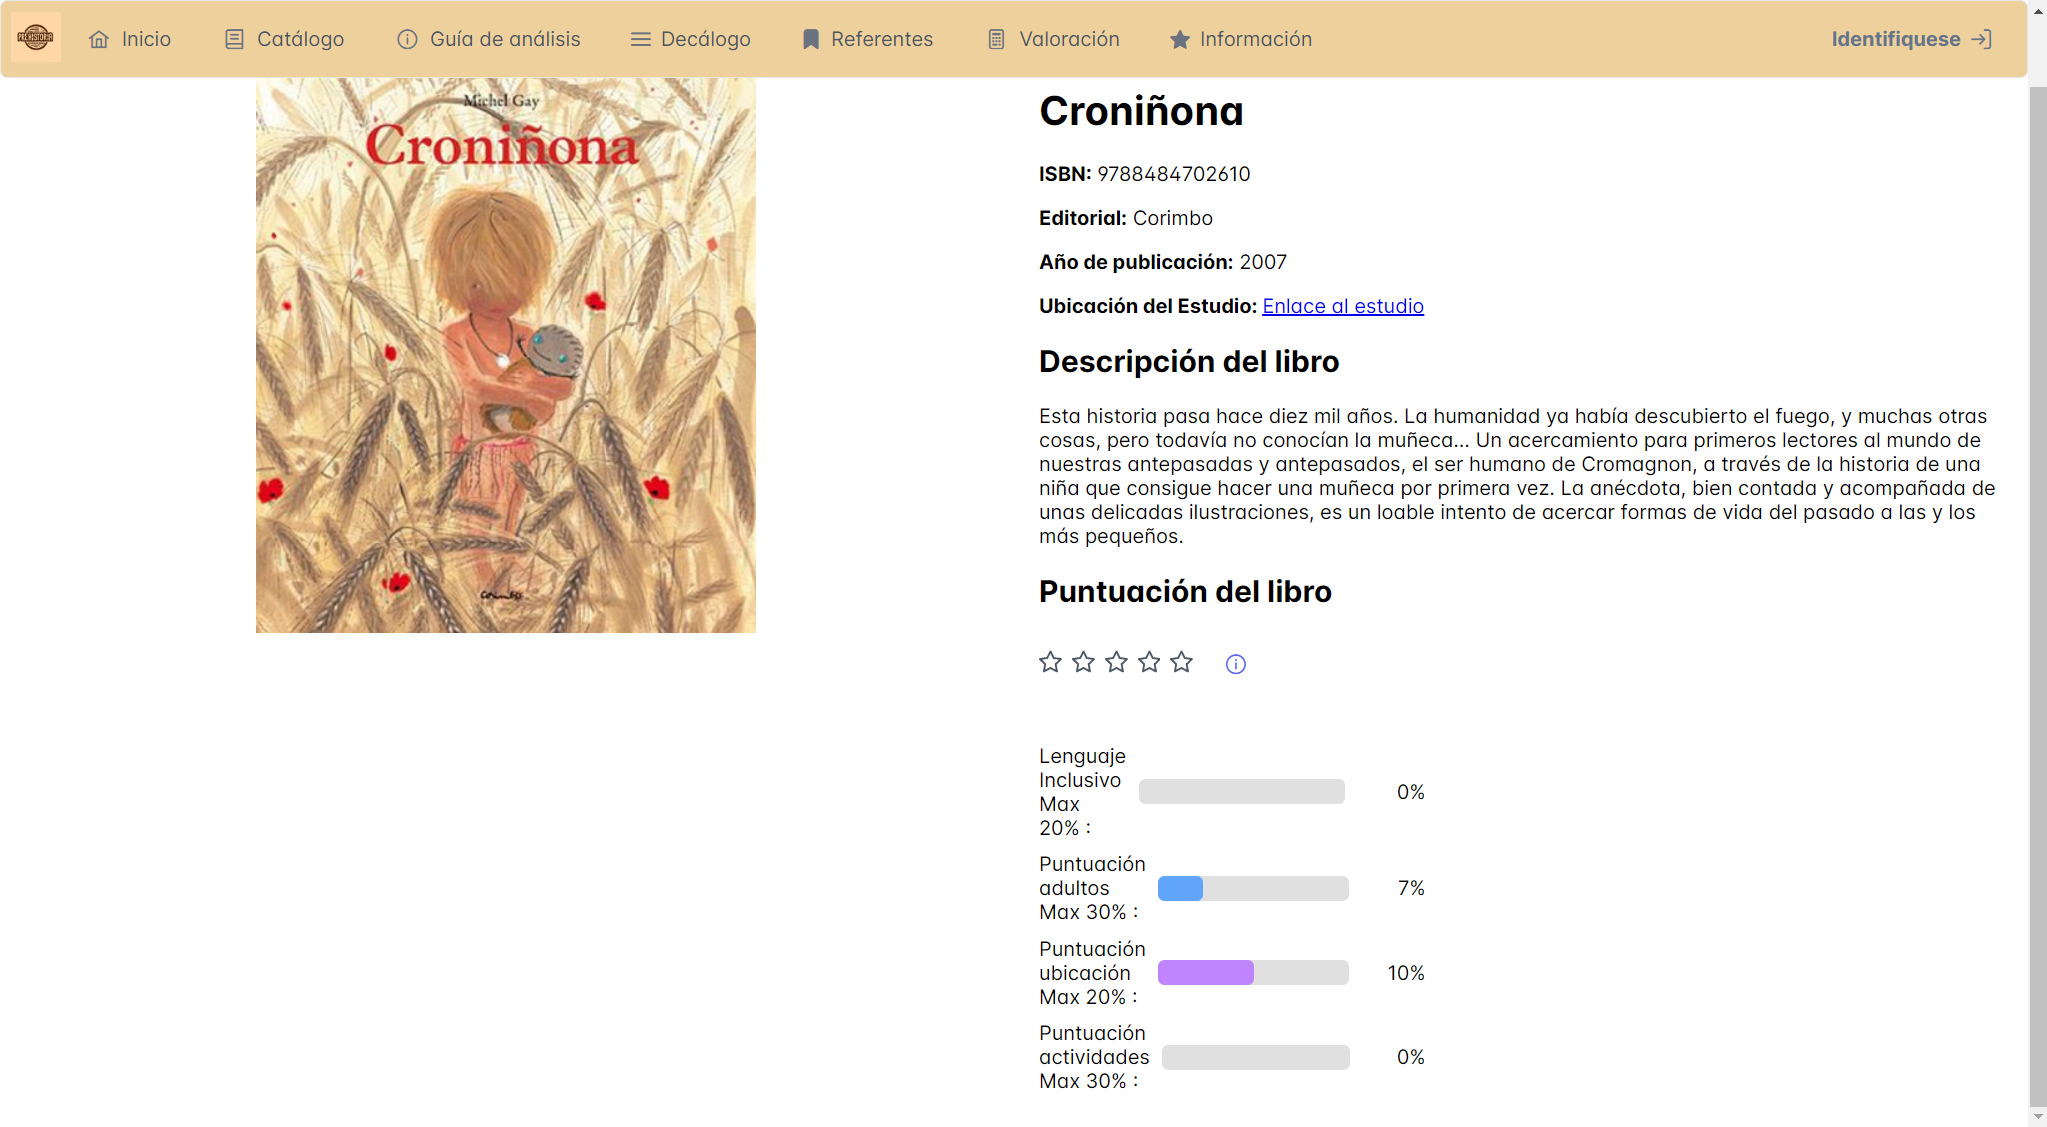
\includegraphics[width=1\linewidth]{Imagenes/ManualMasInfo.png}
    \caption{Más información de un libro}
    \label{Más información de un libro}
\end{figure}
\FloatBarrier

\subsection{Sugerir un libro}
Prehistoria en Igualdad permite a los usuarios realizar recomendaciones al personal de administración para que agreguen nuevos libros al catálogo que puedan ser interesantes de cara a los objetivos de esta aplicación.

Para realizar una sugerencia de un libro:
\begin{itemize}
    \item Entrar en el apartado de catálogo
    \item Pulsar el botón con el icono de un '+' situado abajo a la izquierda.
    \item Rellenar el formulario con los campos solicitados y enviar.
\end{itemize}
\begin{figure}[h]
    \centering
    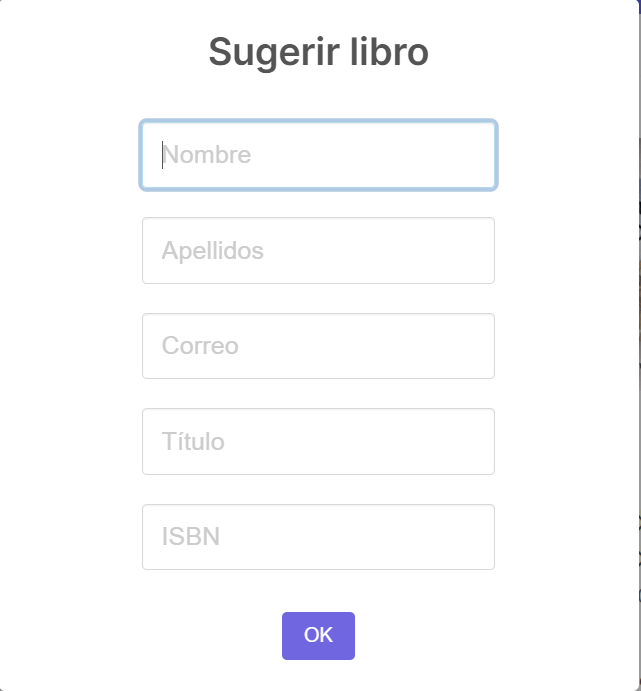
\includegraphics[width=0.6\linewidth]{Imagenes/ManualSugerencia.png}
    \caption{Formulario de sugerencia de libro}
    \label{Formulario de sugerencia de libro}
\end{figure}
\FloatBarrier

\subsection{Realizar una valoración}
Otra de las partes fundamentales de esta aplicación web es la posibilidad que tienen los docentes y familias de realizar sus propias valoraciones de los libros que deseen. Los pasos para realizarla son los siguientes:

\begin{itemize}
    \item Desde el menú acceder a la pestaña de valoración
    \item Rellenar los campos existentes utilizando como base la guía de análisis
    \item Pulsar el botón de calcular.
    \item Una vez se realiza el cálculo, aparecerá una modal con el resultado del cálculo y 3 opciones, navegar a la guía de análisis, no guardar la estimación, o guardarla
    \begin{figure}[h]
        \centering
        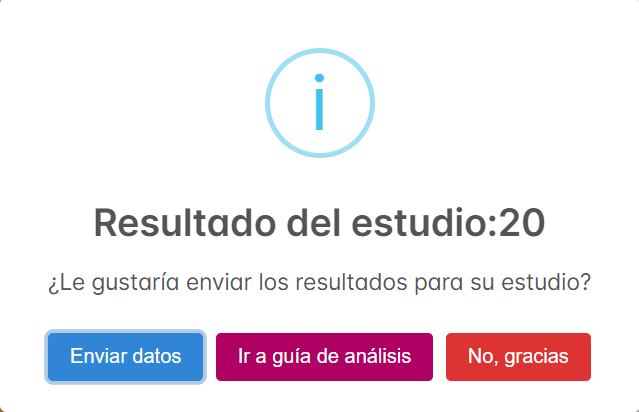
\includegraphics[width=0.6\linewidth]{Imagenes/ManualResultadoValoracion.png}
        \caption{Resultado de valoración}
        \label{Resultado de valoración}
    \end{figure}
    \FloatBarrier
    
    \item En el caso de que se guarde la estimación, aparecerá un formulario para rellenar con los datos personales (opcionales) por si es necesario ponerse en contacto con la persona que la ha realizado.
    \begin{figure}[h]
        \centering
        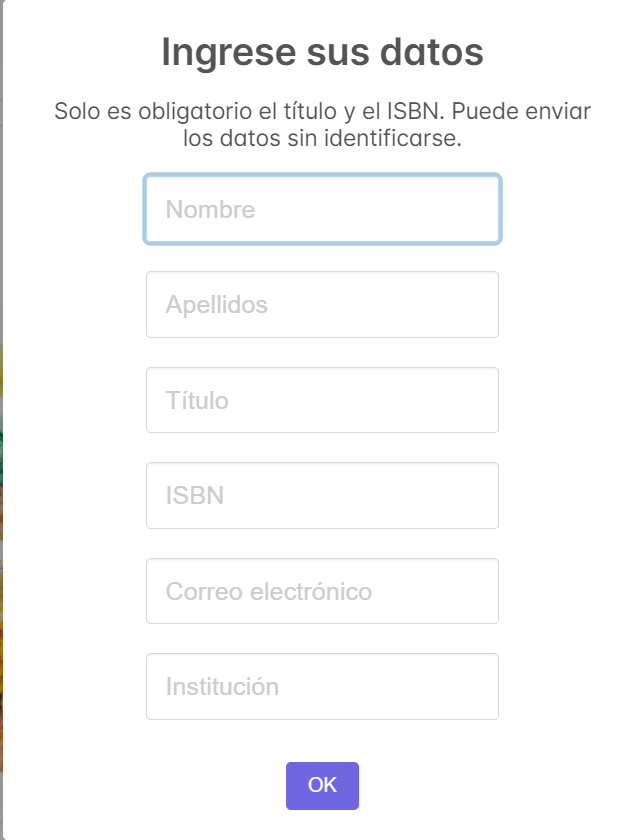
\includegraphics[width=0.5\linewidth]{Imagenes/ManualGuardarValoracion.png}
        \caption{Guardar valoración}
        \label{Guardar valoración}
    \end{figure}
\end{itemize}
\FloatBarrier

\section{Manual del usuario/a con cuenta y permisos de administración}
Antes de continuar con los siguientes apartados, hay que tener en cuenta que todas las operaciones que se realizan por un usuario sin cuenta las puede realizar un usuario con cuenta, por lo que el manual de la sección anterior es válido también para usuarios y usuarias autenticadas. Además de esta aplicación web, está disponible una cuenta de correo electrónico donde se reciben todas las sugerencias realizadas por los usuarios.

\subsection{Iniciar sesión}
Para poder acceder a la zona de administración para realizar todas las operaciones de gestión, han de seguirse los siguientes pasos:
\begin{itemize}
    \item Se selecciona en el menú superior el botón Identifíquese.
    \item Se rellena el campo de usuario y de contraseña para iniciar sesión.
    \begin{figure}[h]
        \centering
        \includegraphics[width=0.6\linewidth]{Imagenes/ManualInicioSesión.png}
        \caption{Manual de Inicio de sesión}
        \label{Manual de Inicio de sesión}
    \end{figure}
    \FloatBarrier
    \item Si se ha iniciado sesión correctamente se redirigirá al catálogo, y en el menú superior, donde se encontraba el botón de identifíquese aparecerá el nombre del usuario y un desplegable que permite acceder al panel de administración y cerrar sesión.
\end{itemize}
\begin{figure}[h]
        \centering
        
\includegraphics[width=0.4\linewidth]{Imagenes/MenuNombreAdmin.png}
        \caption{Cambio de botón Inicio de sesión}
        \label{Cambio de botón Inicio de sesión}
    \end{figure}
    \FloatBarrier

\subsection{Consultar estadísticas de la aplicación web}
Actualmente todo el equipo de administración tiene a su disposición unas métricas mensuales que muestran distintos elementos informativos para consultar de manera gráfica el estado de la aplicación.
A este apartado se accede desde el botón del panel de administrador.
\begin{figure}
    \centering
    \includegraphics[width=1\linewidth]{Imagenes/ManualEstadísticas.png}
    \caption{Estadísticas de administración}
    \label{Estadísticas de administración}
\end{figure}

La información que muestran estas estadísticas es la siguiente:
\begin{itemize}
    \item El primer gráfico muestra el número de visitas totales que se ha tenido este mes entre todos los libros y las visitas del libro más popular.
    \item En el segundo gráfico se puede observar el número de usuarios/as registradas en la aplicación.
    \item El tercer gráfico muestra con gráficos de líneas el número de libros existentes, sugerencias enviadas y estimaciones realizadas cada mes.
    \item El cuarto elemento es una tarjeta donde se indica cuál ha sido el libro más popular.
    \items
\end{itemize}
Cabe destacar que existe la opción de filtrar los datos para acotar los datos en una franja temporal determinada. Por motivos de diseño el máximo de meses a mostrar son 12.

\subsection{Gestión de personas usuarias}
Este apartado es el encargado de dar todas las herramientas que necesite el equipo de administración para tener un control total de quién puede formar parte o no de ese equipo.

Los pasos para realizar una operación en este apartado son los siguientes:
\begin{itemize}
    \item Acceder al panel de administración desde el menú superior.
    \item Desplegar el menú lateral disponible en el menú de administración y seleccionar 'gestión de personas'.
    \item La aplicación muestra las cuentas existentes.
    \item Si se desea crear un nuevo usuario/a:
    \begin{enumerate}
        \item Hacer click en el botón de nuevo usuario.
        \item Rellenar el formulario que se ha desplegado con un nombre, correo y el rol deseado. Si no se selecciona rol, se establece uno predefinido.
        \item Si se ha creado correctamente, aparecerá una modal indicando la contraseña temporal de esa cuenta.
    \end{enumerate}
    \item Si se desea modificar un usuario/a  existente:
    \begin{enumerate}
        \item Hacer click en el lápiz correspondiente a ese usuario/a.
        \item Modificar el formulario que se ha desplegado autocompletado con el nombre, correo y el rol asignado.
        \item Si se ha modificado correctamente, aparecerá una modal indicando éxito en la operación.
    \end{enumerate}
    \item Si se desea eliminar un usuario/a:
    \begin{enumerate}
        \item Hacer click en la papelera correspondiente a ese usuario/a.
        \item Confirmar en la modal la operación por seguridad.
        \item Si se ha eliminado correctamente, aparecerá una modal indicando éxito en la operación.
    \end{enumerate}
\end{itemize}
\begin{figure}[h]
    \centering
    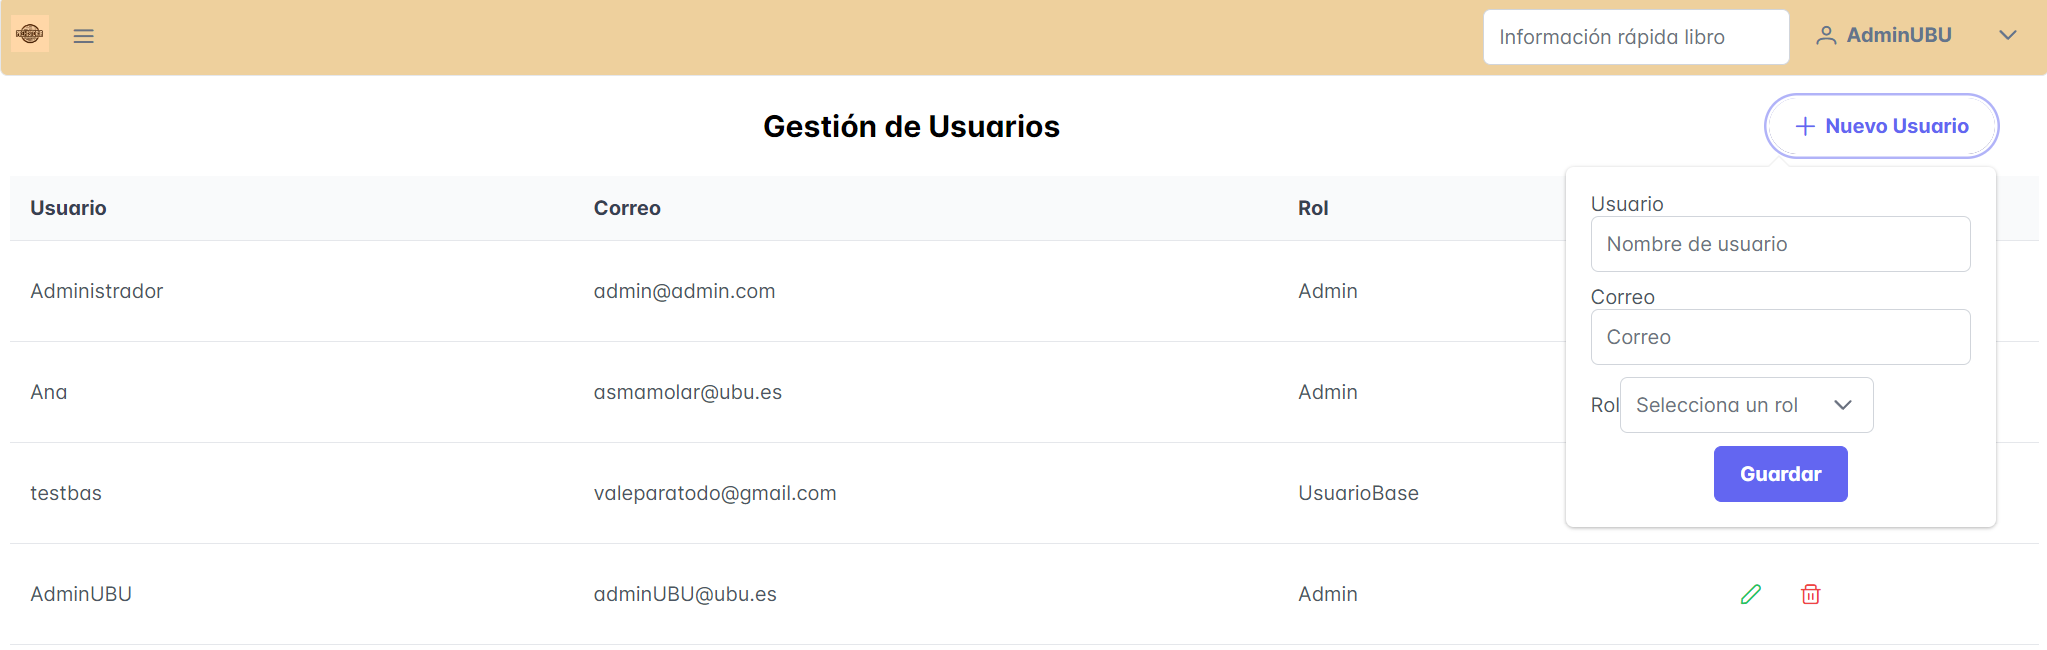
\includegraphics[width=1\linewidth]{Imagenes/ManualUsuarios.png}
    \caption{Operaciones en gestión de usuarios/as}
    \label{Operaciones en gestión de usuarios/as}
\end{figure}
\FloatBarrier

\subsection{Gestión de roles}
Para poder gestionar la autorización de acceso a ciertas funcionalidades de la aplicación, se ha diseñado un sistema de permisos utilizando roles que limitan estas acciones de manera dinámica.

\begin{itemize}
    \item Acceder al panel de administración desde el menú superior.
    \item Desplegar el menú lateral disponible en el menú de administración y seleccionar 'gestión de roles'.
    \item La aplicación muestra los roles existentes.
    \item Si se desea crear un nuevo rol:
    \begin{enumerate}
        \item Hacer click en el botón de nuevo usuario.
        \item Introducir el nombre deseado.
        \item Si se ha creado correctamente, aparecerá una modal el éxito de la operación.
    \end{enumerate}
    \item Si se desea modificar un rol existente:
    \begin{enumerate}
        \item Hacer click en el lápiz correspondiente a ese rol.
        \item Introducir el nuevo nombre de rol deseado.
        \item Si se ha modificado correctamente, aparecerá una modal indicando éxito en la operación.
    \end{enumerate}
    \item Si se desea eliminar un rol:
    \begin{enumerate}
        \item Hacer click en la papelera correspondiente a ese rol.
        \item Confirmar en la modal la operación por seguridad.
        \item Si se ha eliminado correctamente, aparecerá una modal indicando éxito en la operación.
    \end{enumerate}

    \begin{figure}[h]
        \centering
        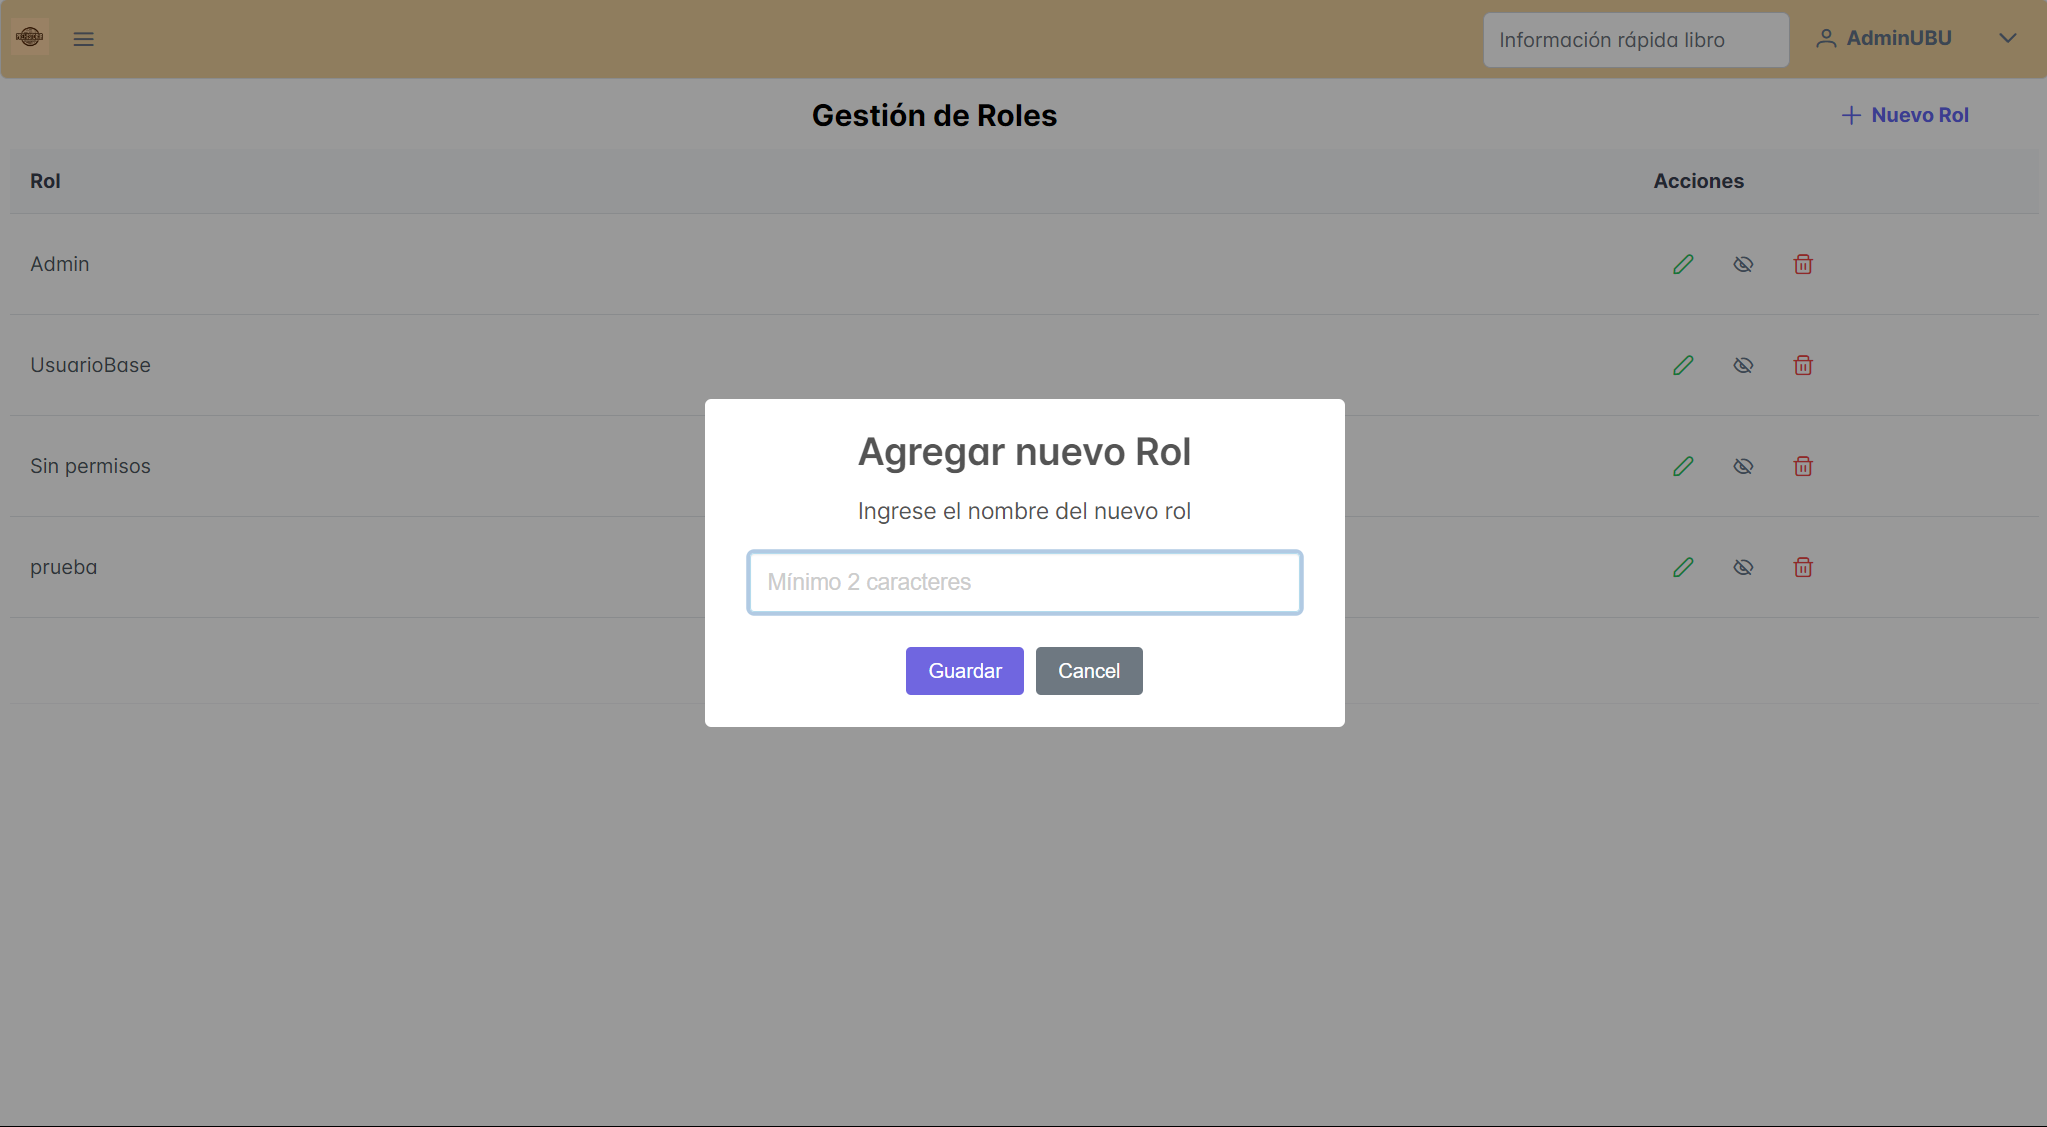
\includegraphics[width=1\linewidth]{Imagenes/ManualRol.png}
        \caption{Operación agregar rol en gestión de roles}
        \label{Operación agregar rol en gestión de roles}
    \end{figure}
    \FloatBarrier

    \item Si se desean gestionar los permisos correspondientes a un rol, ha de seleccionarse el icono del ojo en el rol deseado.
    \item Activar y desactivar los permisos asociados a ese rol y guardar cambios.
\end{itemize}
\begin{figure}[h]
    \centering
    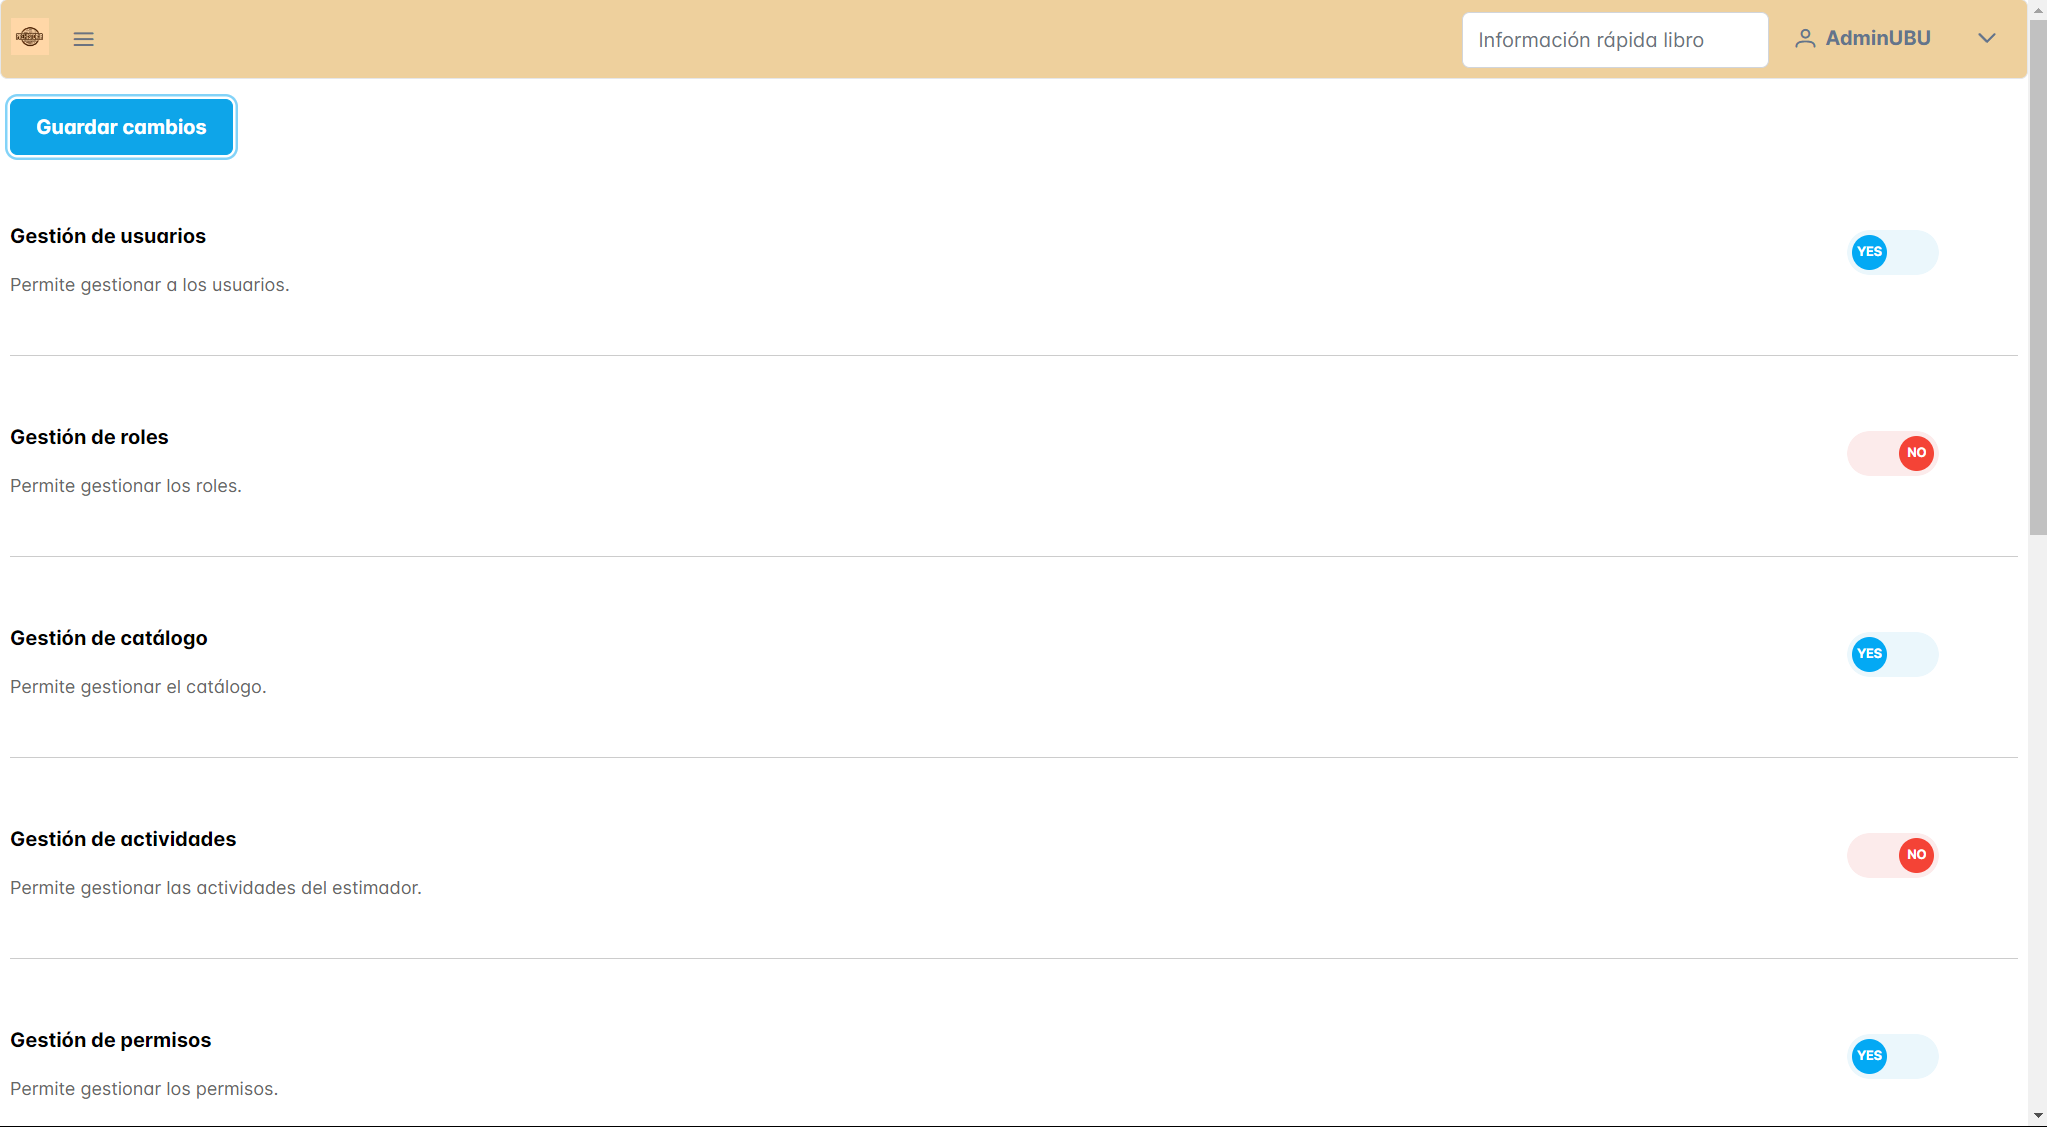
\includegraphics[width=1\linewidth]{Imagenes/ManualPermisos.png}
    \caption{Permisos de un rol}
    \label{Permisos de un rol}
\end{figure}
\FloatBarrier


\subsection{Gestión de colaboradores}
Los colaboradores de esta aplicación web son todos aquellos usuarios/as que han realizado una valoración de un libro la cuál aporte datos objetivos y se considere que ese libro se puede incluir en el catálogo. Para gestionar los colaboradores existentes se han de realizar los siguientes pasos.
\begin{itemize}
    \item Acceder al panel de administración desde el menú superior.
    \item Desplegar el menú lateral ubicado en el menú de administración y seleccionamos 'gestión de colaboradores'.
    \item La aplicación muestra los colaboradores existentes.
    \item Si se desea agregar un nuevo colaborador:
    \begin{enumerate}
        \item Hacer click en el botón Nuevo colaborador.
        \item Rellenar el desplegable con los campos pedidos.
        \item Guardar los cambios.
    \end{enumerate}
    \item Si se desea editar un colaborador:
    \begin{enumerate}
        \item Hacer click en el lápiz correspondiente al colaborador.
        \item Modificar el desplegable con los campos deseados.
        \item Guardar los cambios.
    \end{enumerate}
    \item Si se desea eliminar un colaborador:
    \begin{enumerate}
        \item Hacer click en la papelera correspondiente.
        \item Confirmar en la modal la operación.
    \end{enumerate}
\end{itemize}
\begin{figure}[h]
    \centering
    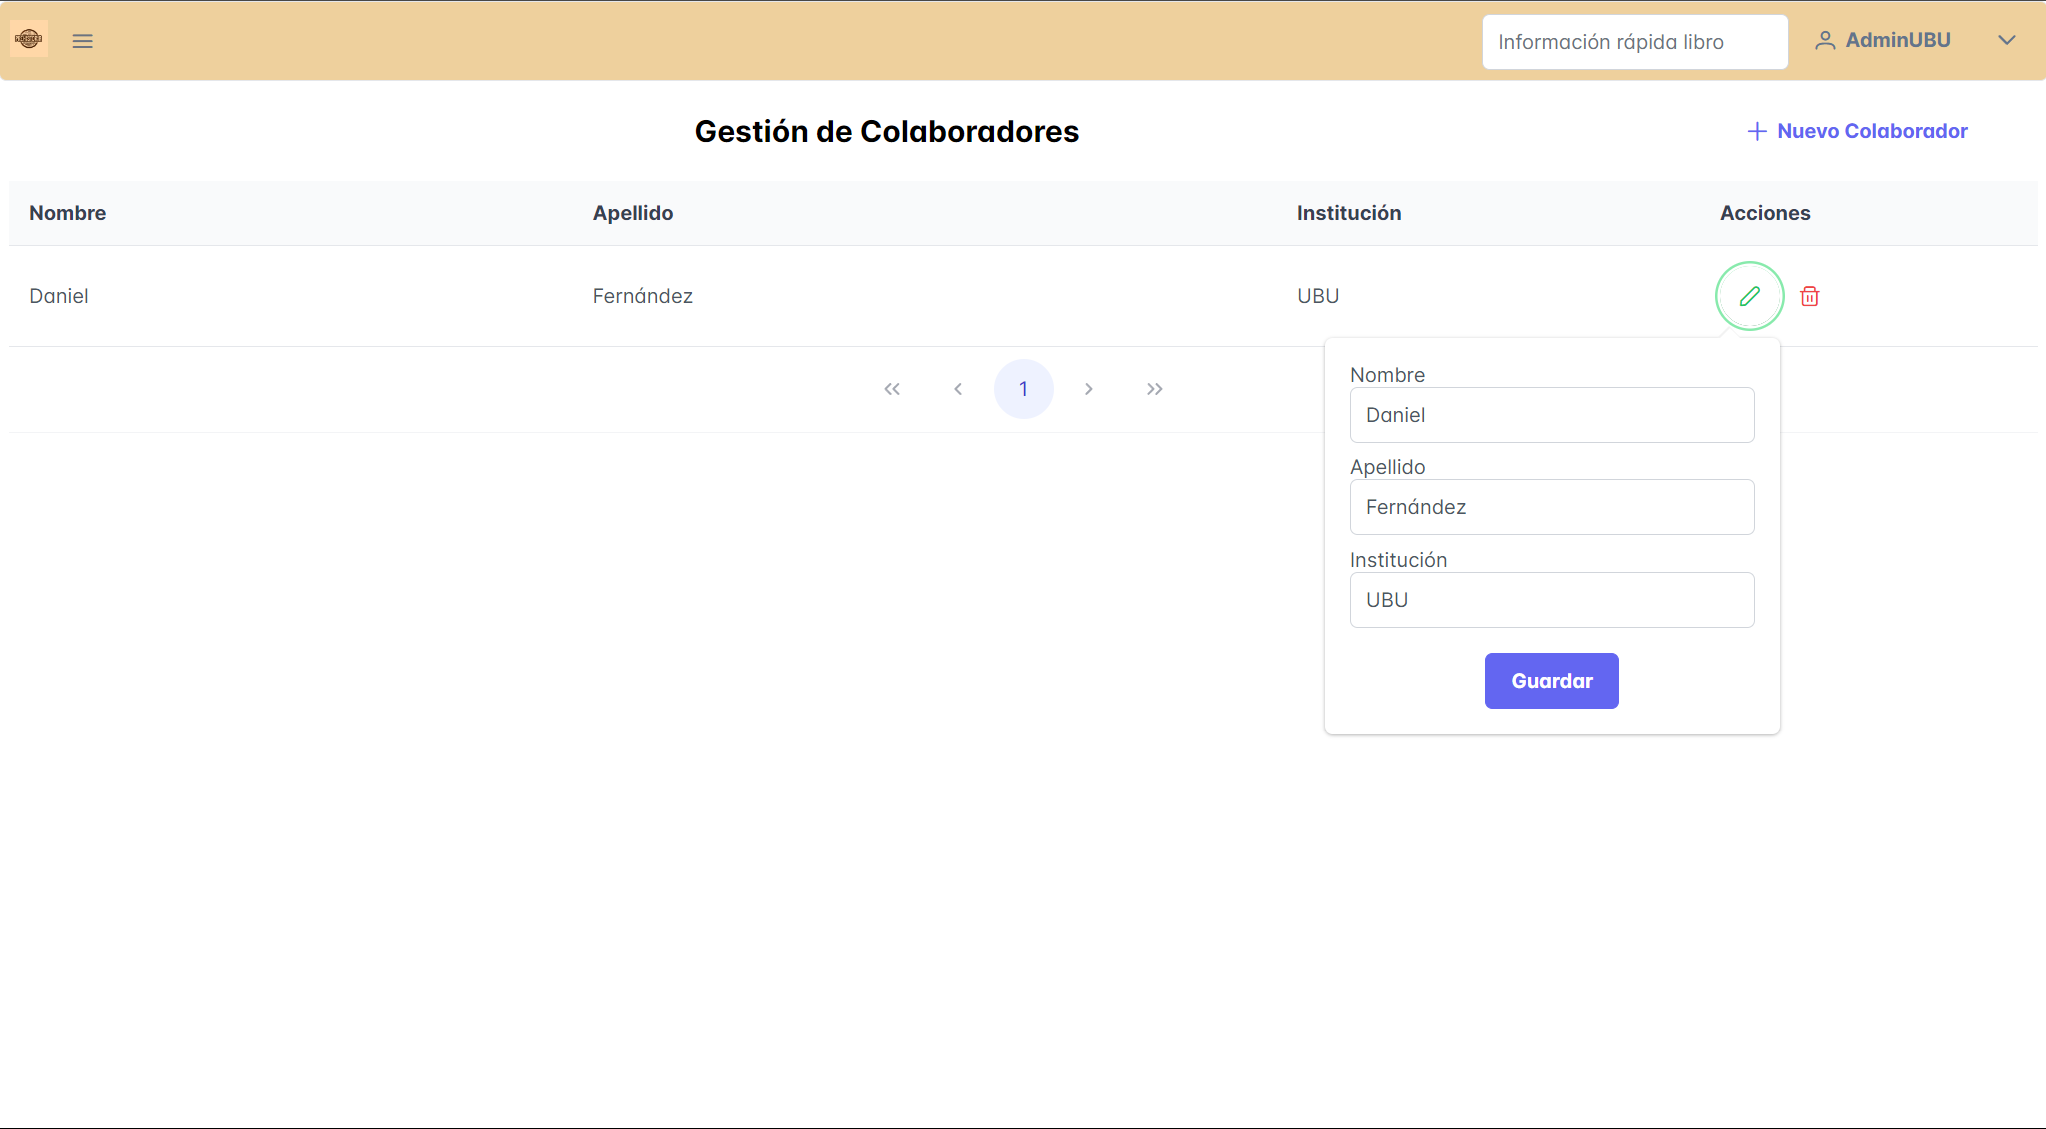
\includegraphics[width=1\linewidth]{Imagenes/ManualColaboraciones.png}
    \caption{Panel de gestión de colaboradores}
    \label{Panel de gestión de colaboradores}
\end{figure}
\FloatBarrier

\subsection{Agregar un nuevo libro}
Una de las piezas fundamentales de esta aplicación es el catálogo y todos sus elementos de gestión que lo rodean. Este apartado va dirigido a explicar las 2 maneras existentes en la aplicación de añadir libros en el catálogo.

\subsubsection{Agregar un libro manualmente}
La forma de agregar un libro manualmente es agregando todos los campos de la información del libro a mano, por lo que se tiene que buscar toda la información.
Los pasos son los siguientes:
\begin{itemize}
    \item Acceder al panel de administración desde el menú superior.
    \item Desplegar el menú lateral ubicado en el menú de administración y seleccionamos la opción 'agregar libro'.
    \item La aplicación muestra un formulario completo con todos los datos que han de incluirse para que se reflejen en el catálogo.
    \item Se rellenan todos los campos (Si ubicación del estudio se queda vacío el programa lo va a sustituir por no disponible).
    \item Si se guarda correctamente la aplicación mostrará una modal indicándolo
\end{itemize}
\begin{figure}
    \centering
    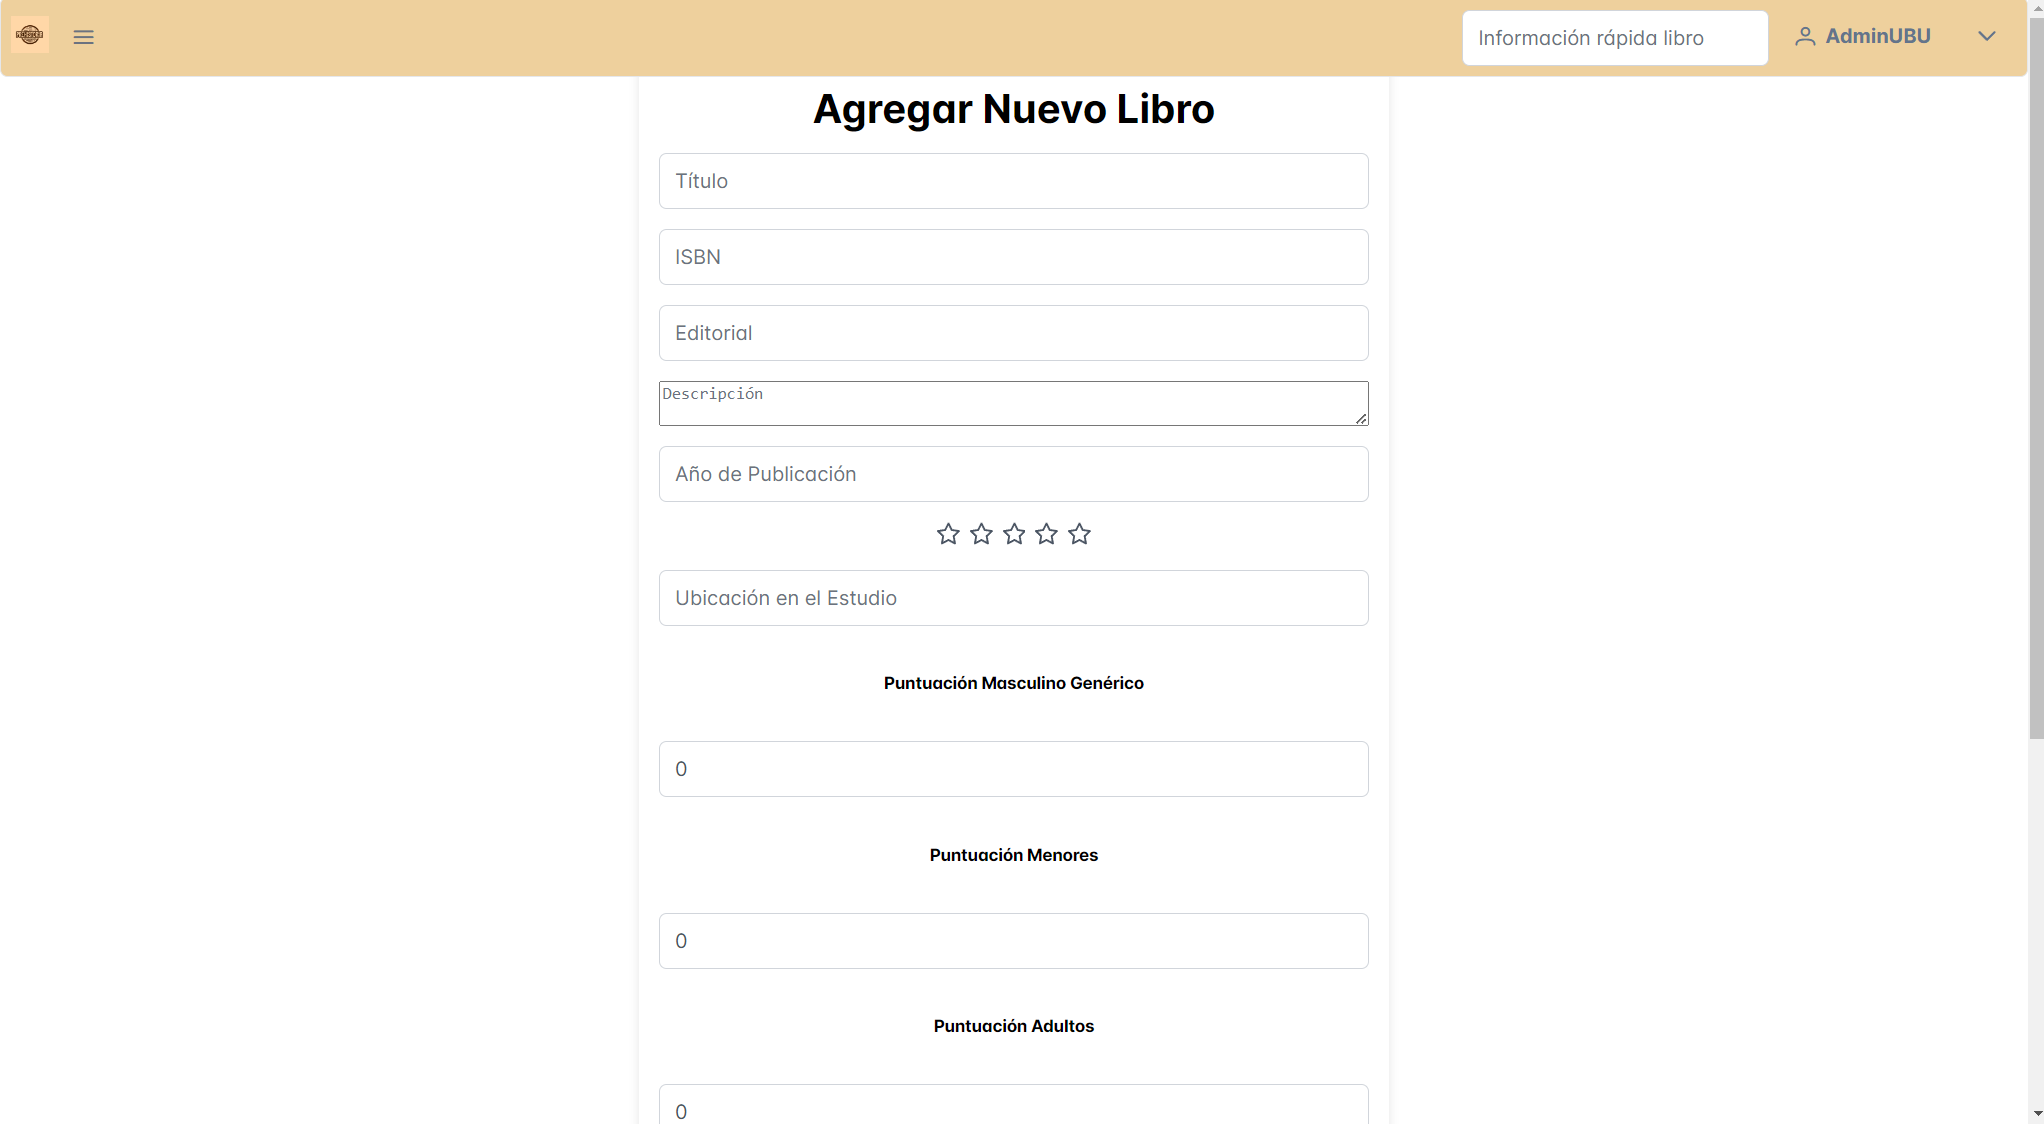
\includegraphics[width=1\linewidth]{Imagenes/ManualAgregar.png}
    \caption{Agregar libro}
    \label{Agregar libro}
\end{figure}

\subsubsection{Agregar un libro automáticamente}
Esta segunda opción ahorra al equipo de administradores el tiempo de encontrar todos los datos utilizando web scraping y la cantidad de datos a rellenar es mucho menor.
Los pasos son los siguientes:

\begin{itemize}
    \item Acceder al panel de administración desde el menú superior.
    \item Desplegar el menú lateral ubicado en el menú de administración y seleccionamos 'agregar libro automáticamente'.
    \item La aplicación muestra una modal donde enviar un título o un ISBN.
    \begin{figure}[h]
        \centering
        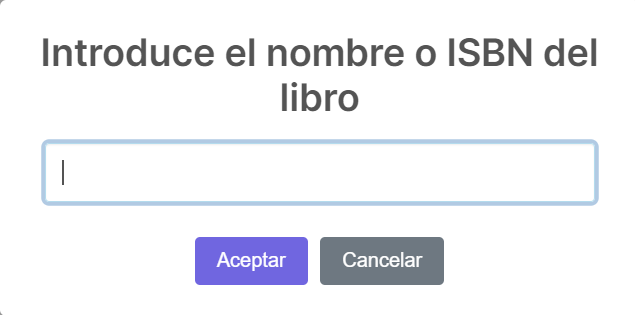
\includegraphics[width=0.5\linewidth]{Imagenes/ManualModalAgregarAuto.png}
        \caption{Modal para agregar automáticamente}
        \label{Modal para agregar automáticamente}
    \end{figure}
    \FloatBarrier
    \item Al enviar esa solicitud aparece una pantalla de carga mientras se buscan posibles libros.
    \item Al terminar la carga aparecerá la información más parecida a la petición realizada en base a 3 fuentes. Abajo del todo aparecerá un botón para ir a agregar un libro manualmente, un botón por cada una de las fuentes para escoger la información de la misma, o un apartado que permite combinar la información de las tres fuentes.
    \begin{figure}[h]
        \centering
        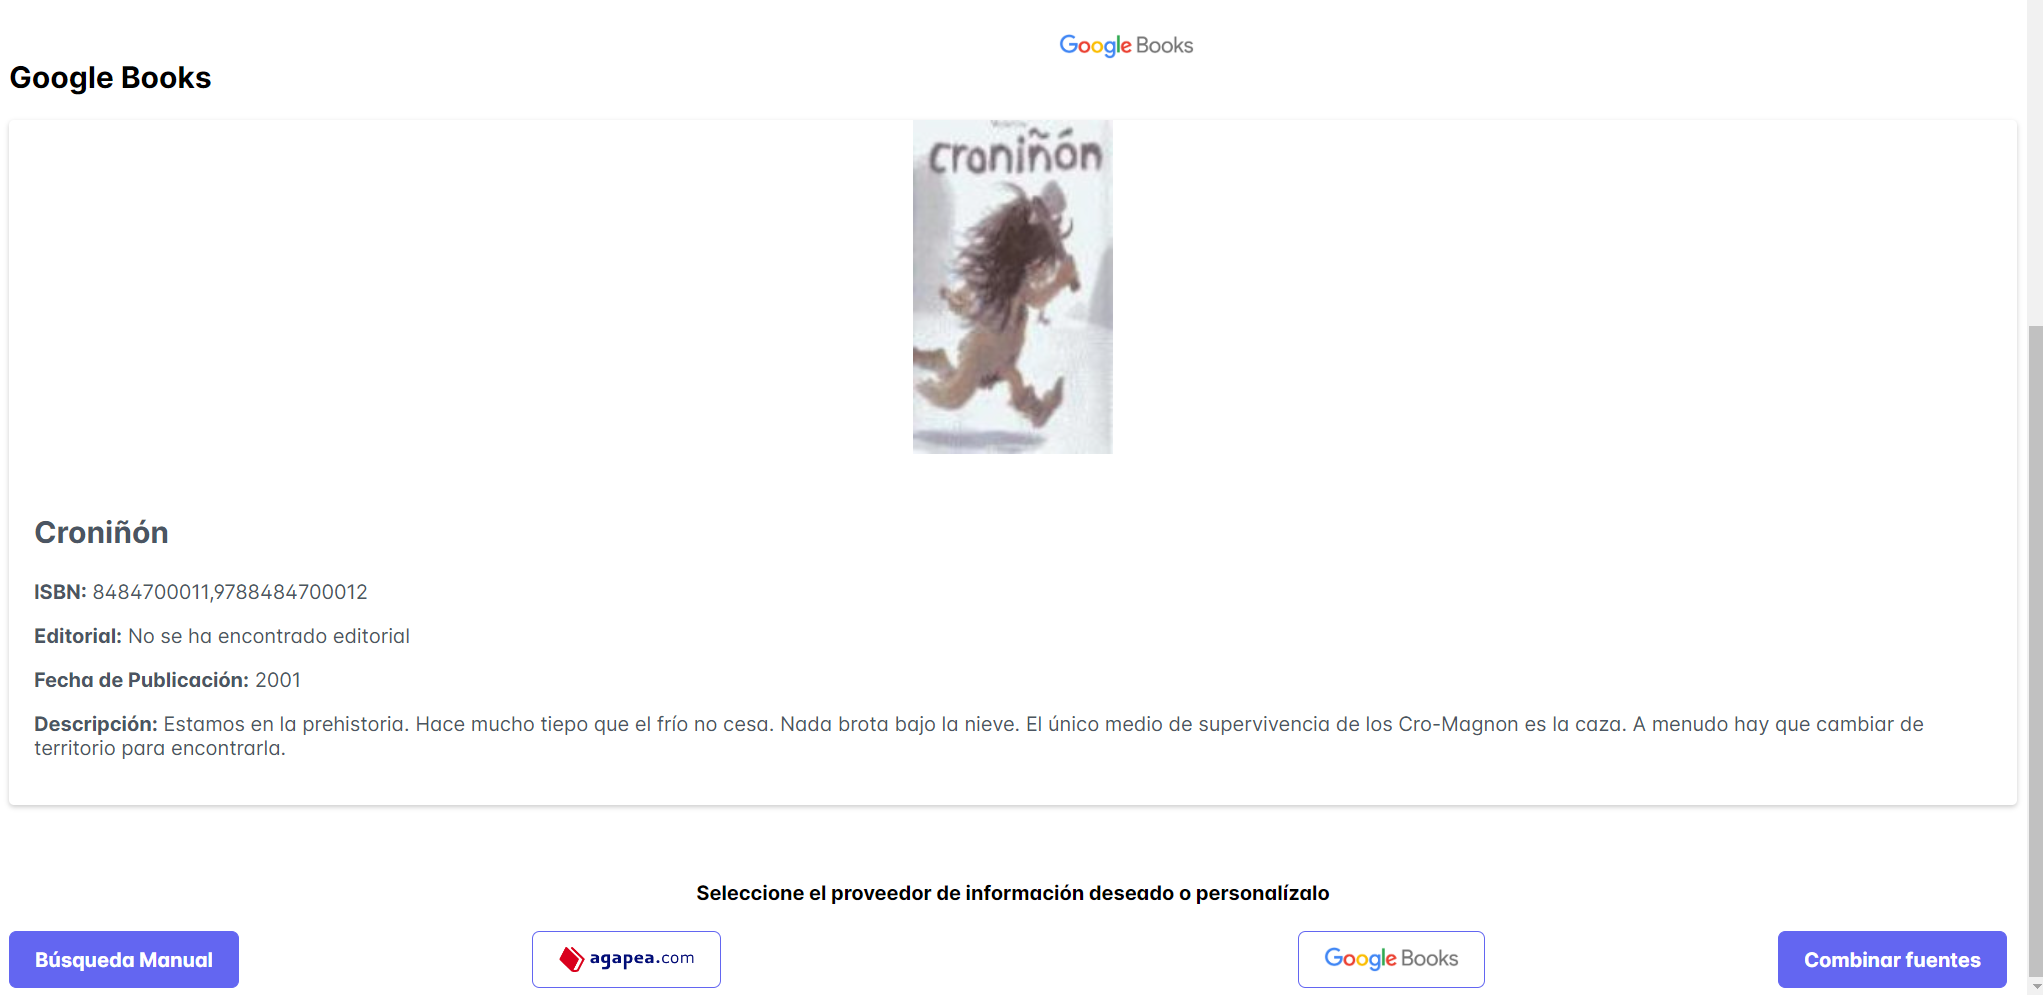
\includegraphics[width=1\linewidth]{Imagenes/ManualSeleccionFuente.png}
        \caption{Selección de fuente de web scraping}
        \label{Selección de fuente de web scraping}
    \end{figure}
    \FloatBarrier

    \item Si se desea agregar un nuevo libro con fuente exclusiva:
    \begin{enumerate}
        \item Se selecciona el botón de esa fuente.
        \item La aplicación se redirigirá al formulario de agregar libro pero con los campos obtenidos autocompletados.
        \item Guardar los cambios.
    \end{enumerate}
    \item Si se desea agregar un nuevo libro con fuentes combinadas:
    \begin{enumerate}
        \item Hacer click en botón de combinar fuentes.
        \item Aparecerá un formulario con los mismos campos que agregar libro pero con desplegables, conteniendo la información de cada fuente, para así seleccionar en cada campo la deseada.
        \item Guardar los cambios.
    \end{enumerate}
\end{itemize}

\begin{figure}[h]
    \centering
    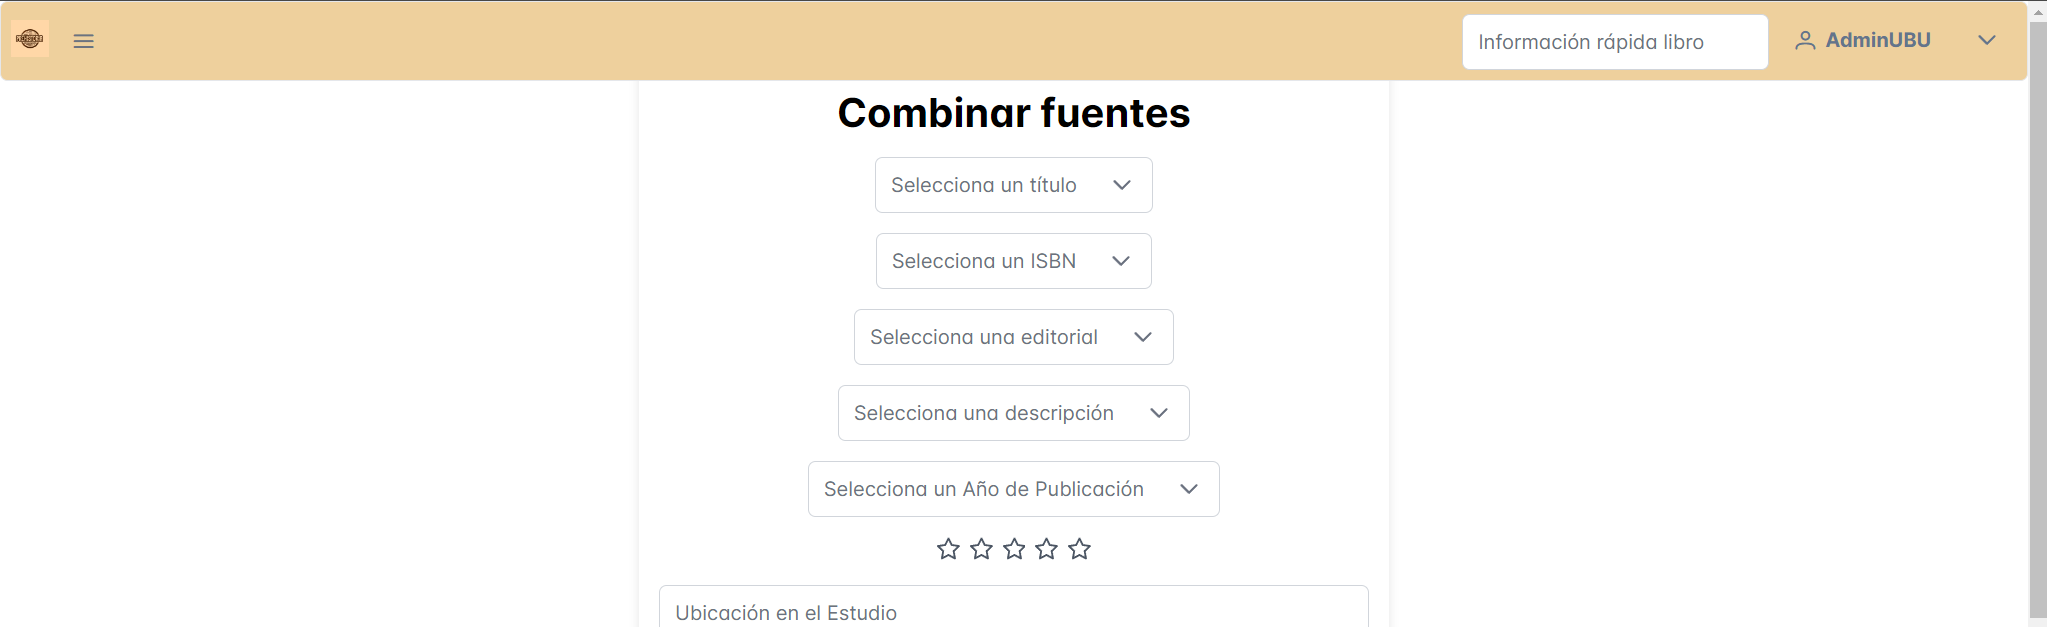
\includegraphics[width=1\linewidth]{Imagenes/ManualCombinar.png}
    \caption{Agregar libro combinando fuentes}
    \label{Agregar libro combinando fuentes}
\end{figure}
\FloatBarrier

\subsection{Gestionar Catálogo}
Además de la herramienta de agregar, el catálogo tiene opciones de editar y eliminar, los pasos para realizar estas operaciones son las siguientes:

\begin{itemize}
    \item Acceder al panel de administración desde el menú superior.
    \item Desplegar el menú lateral ubicado en el menú de administración y seleccionamos 'gestión de catálogo'.
    \item Si se desea editar un libro:
    \begin{enumerate}
        \item Hacer click en el lápiz correspondiente al libro.
        \item Modificar el libro con los campos deseados.
        \item Guardar los cambios.
    \end{enumerate}
    \item Si se desea eliminar un libro:
    \begin{enumerate}
        \item Hacer click en la papelera correspondiente.
        \item Confirmar en la modal la operación.
    \end{enumerate}
\end{itemize}

Finalmente, existe un icono de información en cada libro que redirige a la información del libro seleccionado.
\begin{figure}[h]
    \centering
    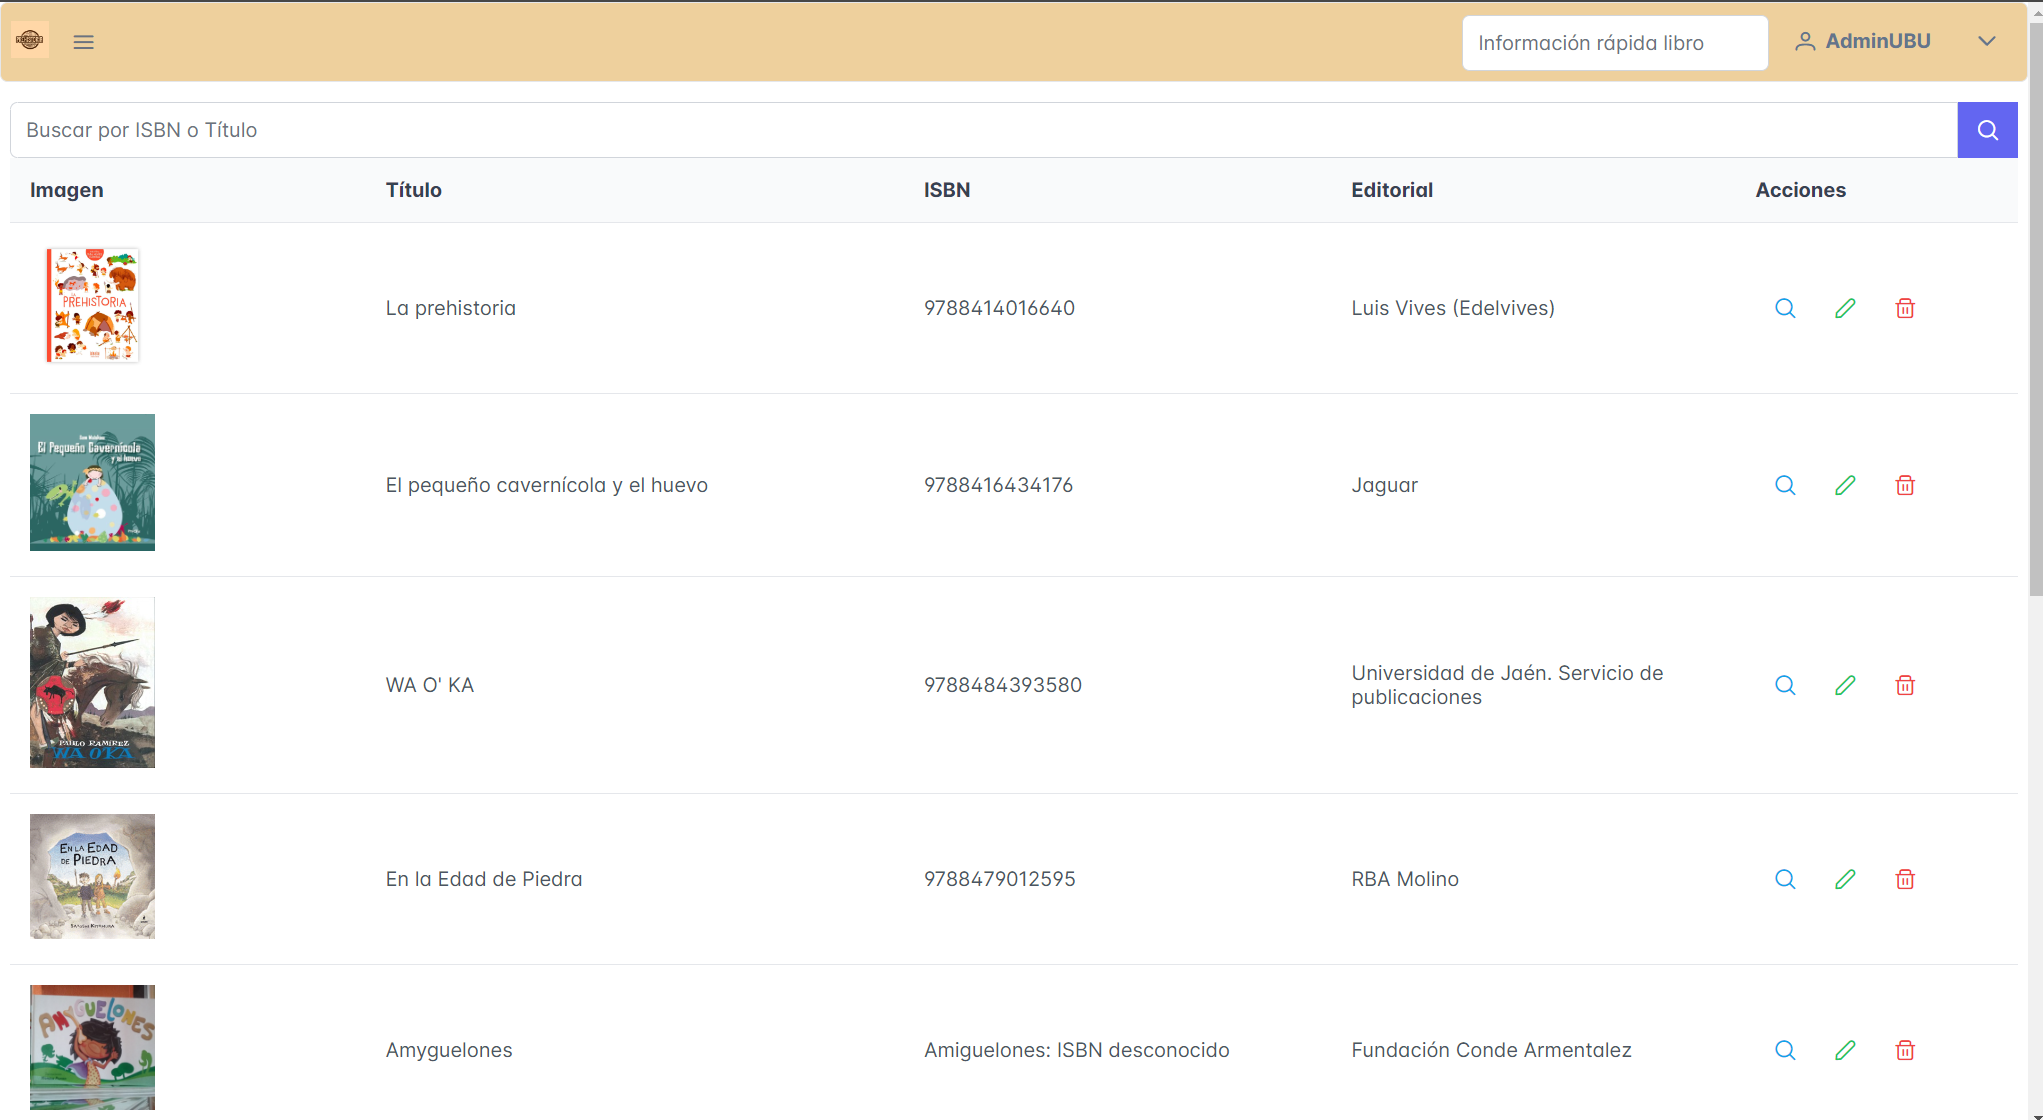
\includegraphics[width=1\linewidth]{Imagenes/ManualGestionCatalogo.png}
    \caption{Pantalla gestión del catálogo}
    \label{Pantalla gestión del catálogo}
\end{figure}
\FloatBarrier

\subsection{Importar y exportar el catálogo}
Para facilitar las labores de agregar libros ya analizados y poder mantener copias de seguridad, se ha facilitado una característica de la aplicación web que permite realizar estas operaciones. A continuación se detallan los pasos:

\begin{itemize}
    \item Acceder al panel de administración desde el menú superior.
    \item Desplegar el menú lateral ubicado en el menú de administración y seleccionamos 'importación o exportación'.
    \item Si se desea importar:
    \begin{enumerate}
        \item Se selecciona el archivo a cargar (Tiene que ser xlsx o csv con separador ;).
    \end{enumerate}
    \item Si se desea exportar:
    \begin{enumerate}
        \item Seleccionar en la modal la extensión con la que se desea exportar.
    \end{enumerate}
\end{itemize}

Es importante mencionar que los archivos a cargar han de incluir todas las siguientes columnas (separadas por ; ):
\begin{itemize}
    \item ID
    \item Título
    \item ISBN
    \item Editorial
    \item Descripción
    \item Año de publicación
    \item Puntuación
    \item Ubicación del estudio
    \item URL de la imagen
    \item Visitas mensuales
    \item Visitas totales
    \item Mes de creación
    \item Año de creación
    \item Puntuación Lenguaje genérico
    \item Puntuación Menores
    \item Puntuación Adultos
    \item Puntuación Ubicación
    \item Puntuación Actividades
\end{itemize}

Es importante destacar que para que la importación/exportación funcione correctamente \textbf{el ISBN debe de ir entre comillas dobles y el campo ID debe de ser único}.

\subsection{Gestión de actividades}
En este apartado se permite al equipo de administración modificar según necesiten las actividades mostradas al generar una valoración.
Los pasos son los siguientes:

\begin{itemize}
    \item Acceder al panel de administración desde el menú superior.
    \item Desplegar el menú lateral disponible en el menú de administración y seleccionar 'gestión de actividades'.
    \item La aplicación muestra las actividades existentes.
    \item Si se desea crear una nueva actividad:
    \begin{enumerate}
        \item Hacer click en el botón de nueva actividad.
        \item Introducir el nombre deseado y las categorías deseadas.
        \item Si se ha creado correctamente, aparecerá una modal el éxito de la operación.
    \end{enumerate}
    \item Si se desea modificar una actividad existente:
    \begin{enumerate}
        \item Hacer click en el lápiz correspondiente a esa actividad.
        \item Introducir el nuevo nombre y las categorías a cambiar.
        \item Si se ha modificado correctamente, aparecerá una modal indicando éxito en la operación.
    \end{enumerate}
    \item Si se desea eliminar un rol:
    \begin{enumerate}
        \item Hacer click en la papelera correspondiente a esa actividad.
    \end{enumerate}
\end{itemize}

\begin{figure}[h]
    \centering
    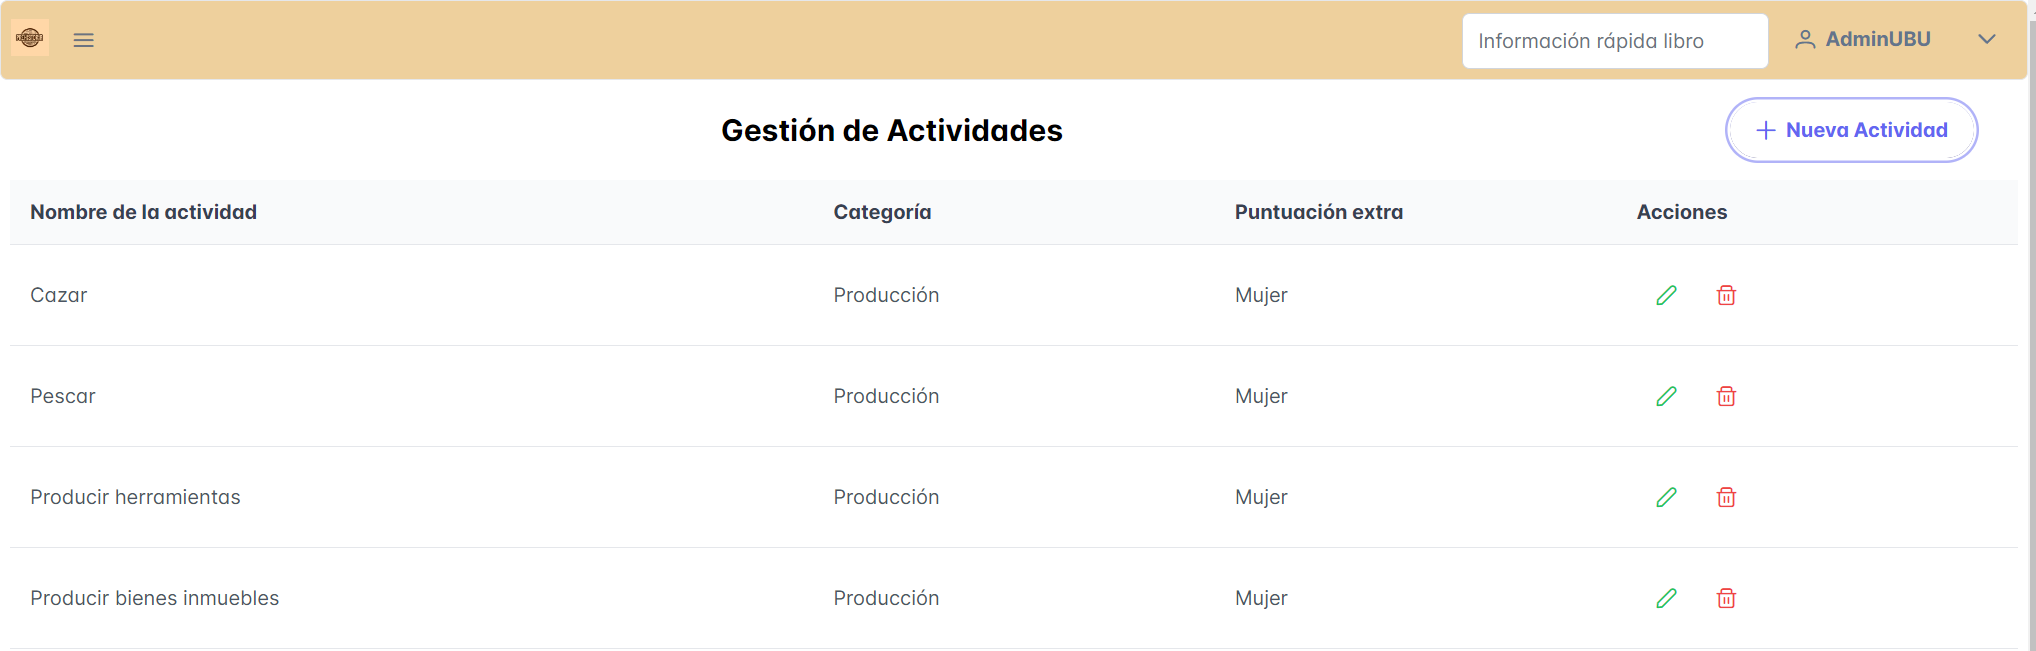
\includegraphics[width=1\linewidth]{Imagenes/ManualActividades.png}
    \caption{Gestión de actividades}
    \label{Gestión de actividades}
\end{figure}
\FloatBarrier

\subsection{Gestionar valoraciones realizadas}
Esta característica de la aplicación permite al equipo de administración observar y eliminar todas las valoraciones que han hecho los usuarios/as.

\begin{itemize}
    \item Acceder al panel de administración desde el menú superior.
    \item Desplegar el menú lateral disponible en el menú de administración y seleccionar 'gestión de valoraciones'.
    \item La aplicación muestra las valoraciones existentes.
    \item Si se desea ver los datos de una valoración existente:
    \begin{enumerate}
        \item Hacer click en el icono de información correspondiente a esa actividad.
        \item Se muestra una modal con toda la información disponible.
    \end{enumerate}
    \item Si se desea eliminar una valoración:
    \begin{enumerate}
        \item Hacer click en la papelera correspondiente a esa valoración.
    \end{enumerate}
    \item Si se desea descargar una valoración:
    \begin{enumerate}
        \item Hacer click en el icono de descargar correspondiente a esa valoración.
        \item Se abrirá una pestaña para ver la dirección de guardado del csv.
    \end{enumerate}
\end{itemize}

\begin{figure}[h]
    \centering
    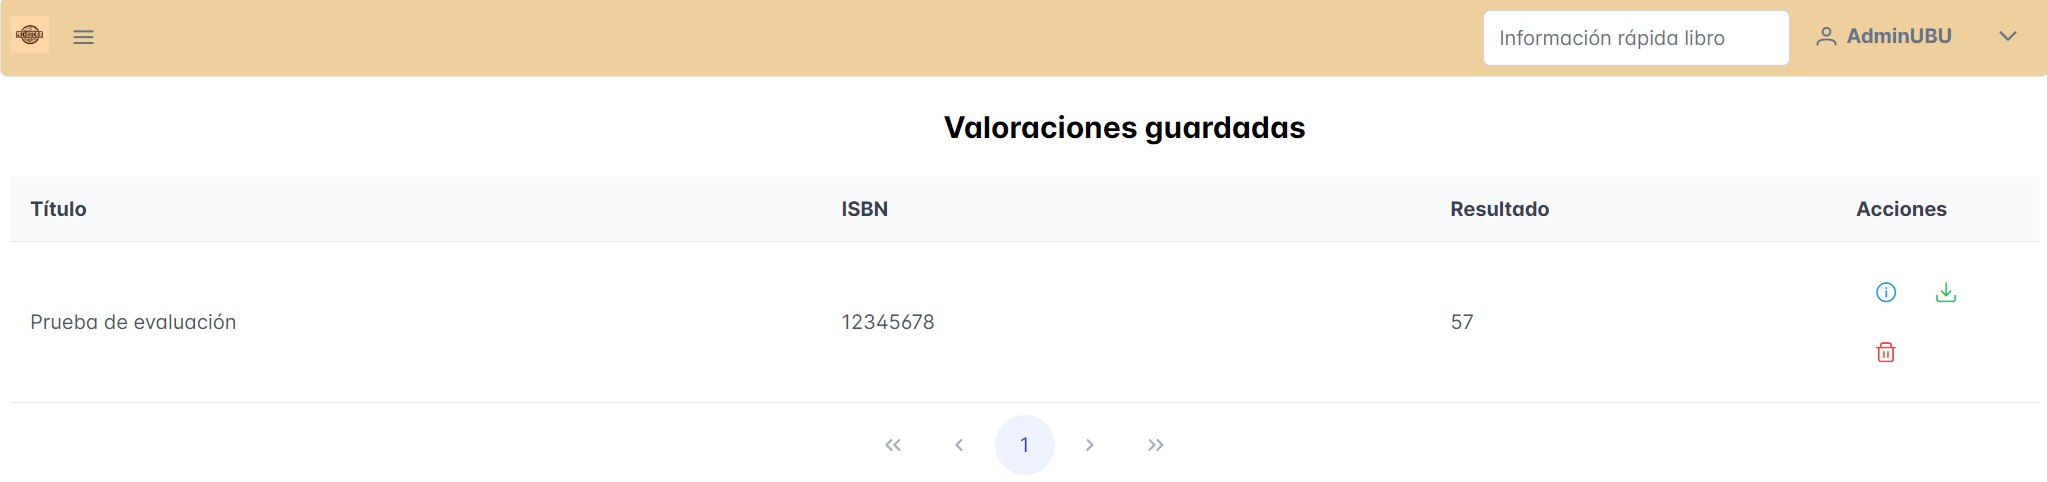
\includegraphics[width=1\linewidth]{Imagenes/ManualValoracionesGuardadas.png}
    \caption{Listado de valoraciones guardadas}
    \label{Listado de valoraciones guardadas}
\end{figure}
\FloatBarrier
\apendice{Anexo de sostenibilización curricular}

\section{Introducción}
Este anexo incluirá una reflexión personal del alumnado sobre los aspectos de la sostenibilidad que se abordan en el trabajo.
Se pueden incluir tantas subsecciones como sean necesarias con la intención de explicar las competencias de sostenibilidad adquiridas durante el alumnado y aplicadas al Trabajo de Fin de Grado.

Más información en el documento de la CRUE \url{https://www.crue.org/wp-content/uploads/2020/02/Directrices_Sosteniblidad_Crue2012.pdf}.

Este anexo tendrá una extensión comprendida entre 600 y 800 palabras.


\bibliographystyle{plain}
\bibliography{bibliografiaAnexos}

\end{document}